\documentclass[journal]{IEEEtran}
\usepackage{amsmath,amssymb,booktabs,graphicx,xcolor,siunitx,tikz,array,multirow,balance}
\usetikzlibrary{arrows.meta,positioning,shapes.geometric,calc,fit}
\usepackage[hidelinks]{hyperref}
% pending.tex -- placeholders for every number and wording that waits on a run.
% Input once in the preamble:  % pending.tex -- placeholders for every number and wording that waits on a run.
% Input once in the preamble:  % pending.tex -- placeholders for every number and wording that waits on a run.
% Input once in the preamble:  \input{pending}
%
% Numbers:   \Gone{key} \Wone{key} \Gsix{key} \NR{key} \Gten{key} \Aone{key} \Athree{key} \Asix{key}
%   -> the value from pending_values.tex (generated from pending_values.csv),
%      or a RED bold placeholder [[ITEM:key]] when the value is not yet known.
% Switches:  \ifitemrun{ITEM}{text if the run is done}{text if it was not run / is pending}
% Wording:   \wordingsel{SLOT}{ITEM}{key}{default}
%   -> picks \defwording{SLOT}{<value of ITEM key>}{...}; uses the pre-registered
%      conservative default when the value is undefined.
% Each unresolved use is logged to pending_report.txt at the end of the run, and
% check_pending.py fails the submission build if any remain.
\makeatletter
\RequirePackage{xcolor}
\def\pend@unresolved{}
\def\statusrun{run}
% ---- run status of each item (overridden by pending_status.tex): run | not_run | pending
\def\status@G1{pending}\def\status@W1{pending}\def\status@G6{pending}\def\status@NR{pending}
\def\status@G10{pending}\def\status@A1{pending}\def\status@A3{pending}\def\status@A6{pending}
\newcommand{\pendingdef}[3]{\expandafter\gdef\csname pend@#1@#2\endcsname{#3}}
\newcommand{\pendingstatus}[2]{\expandafter\gdef\csname status@#1\endcsname{#2}}
\newcommand{\pendingnum}[2]{%
  \ifcsname pend@#1@#2\endcsname
    \csname pend@#1@#2\endcsname
  \else
    \textcolor{red}{\textbf{[[\texttt{\detokenize{#1:#2}}]]}}%
    \xdef\pend@unresolved{\pend@unresolved #1:#2\noexpand\space}%
  \fi}
\newcommand{\ifitemrun}[3]{%
  \ifcsname status@#1\endcsname
    \expandafter\ifx\csname status@#1\endcsname\statusrun #2\else #3\fi
  \else #3\fi}
\newcommand{\defwording}[3]{\expandafter\gdef\csname wording@#1@#2\endcsname{#3}}
\newcommand{\wordingsel}[4]{%
  \ifcsname pend@#2@#3\endcsname
    \edef\pend@k{\csname pend@#2@#3\endcsname}%
  \else
    \def\pend@k{#4}%
    \xdef\pend@unresolved{\pend@unresolved #2:#3(default=#4)\noexpand\space}%
  \fi
  \ifcsname wording@#1@\pend@k\endcsname
    \csname wording@#1@\pend@k\endcsname
  \else
    \textcolor{red}{\textbf{[[no wording \texttt{\detokenize{#1/}}\texttt{\pend@k}]]}}%
  \fi}
% ---- the per-item macros
\newcommand{\Gone}[1]{\pendingnum{G1}{#1}}
\newcommand{\Wone}[1]{\pendingnum{W1}{#1}}
\newcommand{\Gsix}[1]{\pendingnum{G6}{#1}}
\newcommand{\NR}[1]{\pendingnum{NR}{#1}}
\newcommand{\Gten}[1]{\pendingnum{G10}{#1}}
\newcommand{\Aone}[1]{\pendingnum{A1}{#1}}
\newcommand{\Athree}[1]{\pendingnum{A3}{#1}}
\newcommand{\Asix}[1]{\pendingnum{A6}{#1}}
% ---- generated values and statuses, if present
\IfFileExists{pending_values.tex}{\input{pending_values.tex}}{}
\IfFileExists{pending_status.tex}{\input{pending_status.tex}}{}
\IfFileExists{wording.tex}{\input{wording.tex}}{}
% ---- end-of-run report
\newwrite\pend@report
\AtEndDocument{%
  \immediate\openout\pend@report=pending_report.txt
  \immediate\write\pend@report{\pend@unresolved}%
  \immediate\closeout\pend@report}
\makeatother

%
% Numbers:   \Gone{key} \Wone{key} \Gsix{key} \NR{key} \Gten{key} \Aone{key} \Athree{key} \Asix{key}
%   -> the value from pending_values.tex (generated from pending_values.csv),
%      or a RED bold placeholder [[ITEM:key]] when the value is not yet known.
% Switches:  \ifitemrun{ITEM}{text if the run is done}{text if it was not run / is pending}
% Wording:   \wordingsel{SLOT}{ITEM}{key}{default}
%   -> picks \defwording{SLOT}{<value of ITEM key>}{...}; uses the pre-registered
%      conservative default when the value is undefined.
% Each unresolved use is logged to pending_report.txt at the end of the run, and
% check_pending.py fails the submission build if any remain.
\makeatletter
\RequirePackage{xcolor}
\def\pend@unresolved{}
\def\statusrun{run}
% ---- run status of each item (overridden by pending_status.tex): run | not_run | pending
\def\status@G1{pending}\def\status@W1{pending}\def\status@G6{pending}\def\status@NR{pending}
\def\status@G10{pending}\def\status@A1{pending}\def\status@A3{pending}\def\status@A6{pending}
\newcommand{\pendingdef}[3]{\expandafter\gdef\csname pend@#1@#2\endcsname{#3}}
\newcommand{\pendingstatus}[2]{\expandafter\gdef\csname status@#1\endcsname{#2}}
\newcommand{\pendingnum}[2]{%
  \ifcsname pend@#1@#2\endcsname
    \csname pend@#1@#2\endcsname
  \else
    \textcolor{red}{\textbf{[[\texttt{\detokenize{#1:#2}}]]}}%
    \xdef\pend@unresolved{\pend@unresolved #1:#2\noexpand\space}%
  \fi}
\newcommand{\ifitemrun}[3]{%
  \ifcsname status@#1\endcsname
    \expandafter\ifx\csname status@#1\endcsname\statusrun #2\else #3\fi
  \else #3\fi}
\newcommand{\defwording}[3]{\expandafter\gdef\csname wording@#1@#2\endcsname{#3}}
\newcommand{\wordingsel}[4]{%
  \ifcsname pend@#2@#3\endcsname
    \edef\pend@k{\csname pend@#2@#3\endcsname}%
  \else
    \def\pend@k{#4}%
    \xdef\pend@unresolved{\pend@unresolved #2:#3(default=#4)\noexpand\space}%
  \fi
  \ifcsname wording@#1@\pend@k\endcsname
    \csname wording@#1@\pend@k\endcsname
  \else
    \textcolor{red}{\textbf{[[no wording \texttt{\detokenize{#1/}}\texttt{\pend@k}]]}}%
  \fi}
% ---- the per-item macros
\newcommand{\Gone}[1]{\pendingnum{G1}{#1}}
\newcommand{\Wone}[1]{\pendingnum{W1}{#1}}
\newcommand{\Gsix}[1]{\pendingnum{G6}{#1}}
\newcommand{\NR}[1]{\pendingnum{NR}{#1}}
\newcommand{\Gten}[1]{\pendingnum{G10}{#1}}
\newcommand{\Aone}[1]{\pendingnum{A1}{#1}}
\newcommand{\Athree}[1]{\pendingnum{A3}{#1}}
\newcommand{\Asix}[1]{\pendingnum{A6}{#1}}
% ---- generated values and statuses, if present
\IfFileExists{pending_values.tex}{% generated by build_pending.py -- do not edit
}{}
\IfFileExists{pending_status.tex}{% generated by build_pending.py -- do not edit
\pendingstatus{G1}{pending}
\pendingstatus{W1}{pending}
\pendingstatus{G6}{pending}
\pendingstatus{NR}{pending}
\pendingstatus{G10}{pending}
\pendingstatus{A1}{pending}
\pendingstatus{A3}{pending}
\pendingstatus{A6}{pending}
}{}
\IfFileExists{wording.tex}{% wording.tex -- pre-registered wording variants, selected by the verdict of each run.
% Source of truth: paper/proposals/G6 section 4, W1 section 3, NR1 section 4, G10 section 4.
% Key = the value stored as the verdict in pending_values.csv.

% ---- Contribution C2 / abstract clause (G6 verdict: ABJ | ABJ-seed | AB | A | none)
\defwording{C2}{ABJ}{beats all calibrated comparators, including rules re-calibrated by exhaustive search on 500 fresh traces and a table that combines deadline slack, user class and HARQ-process state}
\defwording{C2}{AB}{beats the OLLA family and the single-cue calibrated rules; a calibrated rule that combines the learner's cues matched the learned policy}
\defwording{C2}{A}{beats the OLLA family; against calibrated rules its advantage depends on their calibration budget}
\defwording{C2}{none}{did not survive re-calibration of the comparators}
\defwording{C2}{unrun}{beats the OLLA family and the single-cue calibrated rules (calibrated on 10 to 20 traces)}

% ---- "same-information" may be used only after the G6 combined comparator is beaten
\defwording{SI}{ABJ}{same-information}
\defwording{SI}{AB}{}
\defwording{SI}{A}{}
\defwording{SI}{none}{}
\defwording{SI}{unrun}{}

% ---- NR1 verdict: WIN | CLAIMA | FAIL
\defwording{NR1}{WIN}{The gain does not require class-oracle information in the base rule.}
\defwording{NR1}{CLAIMA}{Part of the margin over calibrated rules comes from the oracle base.}
\defwording{NR1}{FAIL}{With a non-oracle base the residual policy did not beat the OLLA family under realistic HARQ timing; the M1 result relies on the class-oracle base rule.}
\defwording{NR1}{unrun}{The M1 result uses a class-oracle base rule; a non-oracle base was not tested at RTT~8.}

% ---- G10 verdict: ALL | MIXED | NONE   (two cells tested; G10 section 4; never "robust across the range")
\defwording{G10}{ALL}{The gain held at both tested neighbouring operating points (a higher load at the M1 deadline, and a lower load with a looser deadline), including against rules re-calibrated for each cell. Two further grid corners were not tested.}
\defwording{G10}{MIXED}{The gain is operating-point dependent: it held at \Gten{cells_win} but not at \Gten{cells_notwin}. Two further grid corners were not tested.}
\defwording{G10}{NONE}{The result was observed at the M1 operating point only; at the two tested neighbouring points it was not reproduced. Two further grid corners were not tested.}
\defwording{G10}{unrun}{The result is established at one operating point (12~kbit packets, 10-TTI budget); other loads and deadlines were not tested under the corrected scheduler.}

% ---- W1: which condition gives the smaller gain over the OLLA family (cold | warm)
\defwording{W1}{cold}{with loops started at the beginning of each trace}
\defwording{W1}{warm}{after a 200-TTI warm-up}
\defwording{W1}{unrun}{with loops started at the beginning of each trace (cold start)}
}{}
% ---- end-of-run report
\newwrite\pend@report
\AtEndDocument{%
  \immediate\openout\pend@report=pending_report.txt
  \immediate\write\pend@report{\pend@unresolved}%
  \immediate\closeout\pend@report}
\makeatother

%
% Numbers:   \Gone{key} \Wone{key} \Gsix{key} \NR{key} \Gten{key} \Aone{key} \Athree{key} \Asix{key}
%   -> the value from pending_values.tex (generated from pending_values.csv),
%      or a RED bold placeholder [[ITEM:key]] when the value is not yet known.
% Switches:  \ifitemrun{ITEM}{text if the run is done}{text if it was not run / is pending}
% Wording:   \wordingsel{SLOT}{ITEM}{key}{default}
%   -> picks \defwording{SLOT}{<value of ITEM key>}{...}; uses the pre-registered
%      conservative default when the value is undefined.
% Each unresolved use is logged to pending_report.txt at the end of the run, and
% check_pending.py fails the submission build if any remain.
\makeatletter
\RequirePackage{xcolor}
\def\pend@unresolved{}
\def\statusrun{run}
% ---- run status of each item (overridden by pending_status.tex): run | not_run | pending
\def\status@G1{pending}\def\status@W1{pending}\def\status@G6{pending}\def\status@NR{pending}
\def\status@G10{pending}\def\status@A1{pending}\def\status@A3{pending}\def\status@A6{pending}
\newcommand{\pendingdef}[3]{\expandafter\gdef\csname pend@#1@#2\endcsname{#3}}
\newcommand{\pendingstatus}[2]{\expandafter\gdef\csname status@#1\endcsname{#2}}
\newcommand{\pendingnum}[2]{%
  \ifcsname pend@#1@#2\endcsname
    \csname pend@#1@#2\endcsname
  \else
    \textcolor{red}{\textbf{[[\texttt{\detokenize{#1:#2}}]]}}%
    \xdef\pend@unresolved{\pend@unresolved #1:#2\noexpand\space}%
  \fi}
\newcommand{\ifitemrun}[3]{%
  \ifcsname status@#1\endcsname
    \expandafter\ifx\csname status@#1\endcsname\statusrun #2\else #3\fi
  \else #3\fi}
\newcommand{\defwording}[3]{\expandafter\gdef\csname wording@#1@#2\endcsname{#3}}
\newcommand{\wordingsel}[4]{%
  \ifcsname pend@#2@#3\endcsname
    \edef\pend@k{\csname pend@#2@#3\endcsname}%
  \else
    \def\pend@k{#4}%
    \xdef\pend@unresolved{\pend@unresolved #2:#3(default=#4)\noexpand\space}%
  \fi
  \ifcsname wording@#1@\pend@k\endcsname
    \csname wording@#1@\pend@k\endcsname
  \else
    \textcolor{red}{\textbf{[[no wording \texttt{\detokenize{#1/}}\texttt{\pend@k}]]}}%
  \fi}
% ---- the per-item macros
\newcommand{\Gone}[1]{\pendingnum{G1}{#1}}
\newcommand{\Wone}[1]{\pendingnum{W1}{#1}}
\newcommand{\Gsix}[1]{\pendingnum{G6}{#1}}
\newcommand{\NR}[1]{\pendingnum{NR}{#1}}
\newcommand{\Gten}[1]{\pendingnum{G10}{#1}}
\newcommand{\Aone}[1]{\pendingnum{A1}{#1}}
\newcommand{\Athree}[1]{\pendingnum{A3}{#1}}
\newcommand{\Asix}[1]{\pendingnum{A6}{#1}}
% ---- generated values and statuses, if present
\IfFileExists{pending_values.tex}{% generated by build_pending.py -- do not edit
}{}
\IfFileExists{pending_status.tex}{% generated by build_pending.py -- do not edit
\pendingstatus{G1}{pending}
\pendingstatus{W1}{pending}
\pendingstatus{G6}{pending}
\pendingstatus{NR}{pending}
\pendingstatus{G10}{pending}
\pendingstatus{A1}{pending}
\pendingstatus{A3}{pending}
\pendingstatus{A6}{pending}
}{}
\IfFileExists{wording.tex}{% wording.tex -- pre-registered wording variants, selected by the verdict of each run.
% Source of truth: paper/proposals/G6 section 4, W1 section 3, NR1 section 4, G10 section 4.
% Key = the value stored as the verdict in pending_values.csv.

% ---- Contribution C2 / abstract clause (G6 verdict: ABJ | ABJ-seed | AB | A | none)
\defwording{C2}{ABJ}{beats all calibrated comparators, including rules re-calibrated by exhaustive search on 500 fresh traces and a table that combines deadline slack, user class and HARQ-process state}
\defwording{C2}{AB}{beats the OLLA family and the single-cue calibrated rules; a calibrated rule that combines the learner's cues matched the learned policy}
\defwording{C2}{A}{beats the OLLA family; against calibrated rules its advantage depends on their calibration budget}
\defwording{C2}{none}{did not survive re-calibration of the comparators}
\defwording{C2}{unrun}{beats the OLLA family and the single-cue calibrated rules (calibrated on 10 to 20 traces)}

% ---- "same-information" may be used only after the G6 combined comparator is beaten
\defwording{SI}{ABJ}{same-information}
\defwording{SI}{AB}{}
\defwording{SI}{A}{}
\defwording{SI}{none}{}
\defwording{SI}{unrun}{}

% ---- NR1 verdict: WIN | CLAIMA | FAIL
\defwording{NR1}{WIN}{The gain does not require class-oracle information in the base rule.}
\defwording{NR1}{CLAIMA}{Part of the margin over calibrated rules comes from the oracle base.}
\defwording{NR1}{FAIL}{With a non-oracle base the residual policy did not beat the OLLA family under realistic HARQ timing; the M1 result relies on the class-oracle base rule.}
\defwording{NR1}{unrun}{The M1 result uses a class-oracle base rule; a non-oracle base was not tested at RTT~8.}

% ---- G10 verdict: ALL | MIXED | NONE   (two cells tested; G10 section 4; never "robust across the range")
\defwording{G10}{ALL}{The gain held at both tested neighbouring operating points (a higher load at the M1 deadline, and a lower load with a looser deadline), including against rules re-calibrated for each cell. Two further grid corners were not tested.}
\defwording{G10}{MIXED}{The gain is operating-point dependent: it held at \Gten{cells_win} but not at \Gten{cells_notwin}. Two further grid corners were not tested.}
\defwording{G10}{NONE}{The result was observed at the M1 operating point only; at the two tested neighbouring points it was not reproduced. Two further grid corners were not tested.}
\defwording{G10}{unrun}{The result is established at one operating point (12~kbit packets, 10-TTI budget); other loads and deadlines were not tested under the corrected scheduler.}

% ---- W1: which condition gives the smaller gain over the OLLA family (cold | warm)
\defwording{W1}{cold}{with loops started at the beginning of each trace}
\defwording{W1}{warm}{after a 200-TTI warm-up}
\defwording{W1}{unrun}{with loops started at the beginning of each trace (cold start)}
}{}
% ---- end-of-run report
\newwrite\pend@report
\AtEndDocument{%
  \immediate\openout\pend@report=pending_report.txt
  \immediate\write\pend@report{\pend@unresolved}%
  \immediate\closeout\pend@report}
\makeatother

% generated by build_numbers.py -- do not edit. Every value comes from a file listed in numbers_audit.csv.
\newcommand{\NADlCtxEight}{+1.58}%
\newcommand{\NADlCtxSwing}{1.15}%
\newcommand{\NADlCtxZero}{+0.43}%
\newcommand{\NADlFixedEight}{+1.87}%
\newcommand{\NADlFixedSwing}{0.94}%
\newcommand{\NADlFixedZero}{+0.93}%
\newcommand{\NAGpCtxEight}{\ensuremath{-}0.88}%
\newcommand{\NAGpCtxSwing}{0.85}%
\newcommand{\NAGpCtxZero}{\ensuremath{-}1.73}%
\newcommand{\NAGpFixedEight}{\ensuremath{-}0.88}%
\newcommand{\NAGpFixedSwing}{0.85}%
\newcommand{\NAGpFixedZero}{\ensuremath{-}1.73}%
\newcommand{\NActiveHours}{6.3}%
\newcommand{\NAoneAllHi}{+2.62}%
\newcommand{\NAoneAllLo}{+0.62}%
\newcommand{\NAoneAllMar}{+1.59}%
\newcommand{\NAoneAllShare}{100}%
\newcommand{\NAoneEdgeHi}{20}%
\newcommand{\NAoneEdgeLo}{10}%
\newcommand{\NAoneFastHi}{+3.68}%
\newcommand{\NAoneFastLo}{+0.91}%
\newcommand{\NAoneFastMar}{+2.25}%
\newcommand{\NAoneFastShare}{32}%
\newcommand{\NAoneMidHi}{+3.89}%
\newcommand{\NAoneMidLo}{+1.80}%
\newcommand{\NAoneMidMar}{+2.82}%
\newcommand{\NAoneMidShare}{47}%
\newcommand{\NAoneSlowHi}{\ensuremath{-}0.15}%
\newcommand{\NAoneSlowLo}{\ensuremath{-}3.32}%
\newcommand{\NAoneSlowMar}{\ensuremath{-}1.71}%
\newcommand{\NAoneSlowShare}{21}%
\newcommand{\NAsixBaseAckDJain}{\ensuremath{-}0.097}%
\newcommand{\NAsixBaseAckGain}{+44.7}%
\newcommand{\NAsixBaseAckRatio}{1.447}%
\newcommand{\NAsixBaseSchedDJain}{+0.004}%
\newcommand{\NAsixBaseSchedGain}{\ensuremath{-}2.4}%
\newcommand{\NAsixBaseSchedRatio}{0.976}%
\newcommand{\NAsixFixedAckDJain}{\ensuremath{-}0.102}%
\newcommand{\NAsixFixedAckGain}{+42.0}%
\newcommand{\NAsixFixedAckRatio}{1.420}%
\newcommand{\NAsixFixedSchedDJain}{+0.001}%
\newcommand{\NAsixFixedSchedGain}{+0.7}%
\newcommand{\NAsixFixedSchedRatio}{1.007}%
\newcommand{\NAsixGpAckEight}{4.23}%
\newcommand{\NAsixGpAckOne}{2.92}%
\newcommand{\NAsixGpSchedEight}{3.21}%
\newcommand{\NAsixGpSchedOne}{3.29}%
\newcommand{\NAsixJainAckEight}{0.436}%
\newcommand{\NAsixJainAckOne}{0.534}%
\newcommand{\NAsixJainSchedEight}{0.498}%
\newcommand{\NAsixJainSchedOne}{0.494}%
\newcommand{\NAsixOLLAAckDJain}{\ensuremath{-}0.098}%
\newcommand{\NAsixOLLAAckGain}{+43.3}%
\newcommand{\NAsixOLLAAckRatio}{1.433}%
\newcommand{\NAsixOLLASchedDJain}{+0.004}%
\newcommand{\NAsixOLLASchedGain}{\ensuremath{-}2.4}%
\newcommand{\NAsixOLLASchedRatio}{0.976}%
\newcommand{\NAsixTraces}{100}%
\newcommand{\NAthreeCpu}{i5-8350U}%
\newcommand{\NAthreeFwd}{9.01}%
\newcommand{\NAthreeLoop}{2.03}%
\newcommand{\NAthreeRatio}{2.40}%
\newcommand{\NAthreeTti}{830.3}%
\newcommand{\NAthreeTtiFpu}{346.2}%
\newcommand{\NBonfP}{$8.8\times10^{-10}$}%
\newcommand{\NBonfPCtxJ}{1.00}%
\newcommand{\NBonfPCtxJProj}{1.00}%
\newcommand{\NBonfPProj}{$1.1\times10^{-9}$}%
\newcommand{\NBonfPraw}{$9.1\times10^{-13}$}%
\newcommand{\NBonfTests}{972}%
\newcommand{\NBoot}{20\,000}%
\newcommand{\NCalClasses}{6}%
\newcommand{\NCalCtxPasses}{2}%
\newcommand{\NCalCtxTables}{343}%
\newcommand{\NCalFixedCands}{9}%
\newcommand{\NCfgBurnIn}{50}%
\newcommand{\NCfgBurstDb}{9}%
\newcommand{\NCfgCalib}{20}%
\newcommand{\NCfgCalibCtx}{10}%
\newcommand{\NCfgChase}{2.5}%
\newcommand{\NCfgDcorr}{50}%
\newcommand{\NCfgDeadline}{10}%
\newcommand{\NCfgDwellBurst}{120}%
\newcommand{\NCfgDwellCalm}{250}%
\newcommand{\NCfgEpDl}{3000}%
\newcommand{\NCfgEpGp}{800}%
\newcommand{\NCfgEpShort}{800}%
\newcommand{\NCfgEval}{500}%
\newcommand{\NCfgMaxRetx}{3}%
\newcommand{\NCfgNproc}{8}%
\newcommand{\NCfgOllaDown}{0.5}%
\newcommand{\NCfgOllaLim}{10}%
\newcommand{\NCfgOllaTarget}{0.1}%
\newcommand{\NCfgOllaUp}{0.056}%
\newcommand{\NCfgPeriod}{20}%
\newcommand{\NCfgPfAlpha}{0.05}%
\newcommand{\NCfgPkt}{12000}%
\newcommand{\NCfgPktKbit}{12}%
\newcommand{\NCfgRB}{100}%
\newcommand{\NCfgResidBias}{3}%
\newcommand{\NCfgResidPen}{0.02}%
\newcommand{\NCfgRtt}{8}%
\newcommand{\NCfgScored}{150}%
\newcommand{\NCfgSeeds}{10}%
\newcommand{\NCfgShape}{0.5}%
\newcommand{\NCfgSigmaMeas}{1}%
\newcommand{\NCfgSigmaSF}{6}%
\newcommand{\NCfgSpeedMax}{30}%
\newcommand{\NCfgSpeedMin}{3}%
\newcommand{\NCfgTrace}{200}%
\newcommand{\NCfgUsers}{10}%
\newcommand{\NEngineGap}{10.71}%
\newcommand{\NEngineJain}{0.0228}%
\newcommand{\NFairJain}{0.0056}%
\newcommand{\NFairRatio}{1.0010}%
\newcommand{\NFlopsActor}{40\,195}%
\newcommand{\NGMoneCtxAbove}{9}%
\newcommand{\NGMoneCtxBootHi}{+2.53}%
\newcommand{\NGMoneCtxBootLo}{+0.72}%
\newcommand{\NGMoneCtxHierHi}{+2.62}%
\newcommand{\NGMoneCtxHierLo}{+0.62}%
\newcommand{\NGMoneCtxHierNinetyHi}{+2.45}%
\newcommand{\NGMoneCtxHierNinetyLo}{+0.76}%
\newcommand{\NGMoneCtxSeedMax}{+4.41}%
\newcommand{\NGMoneCtxSeedMin}{\ensuremath{-}0.80}%
\newcommand{\NGMoneCtxSign}{0.0107}%
\newcommand{\NGMoneCtxTHi}{+2.68}%
\newcommand{\NGMoneCtxTLo}{+0.48}%
\newcommand{\NGMoneCtxTraceNinetyHi}{+1.95}%
\newcommand{\NGMoneCtxTraceNinetyLo}{+1.22}%
\newcommand{\NGMoneFPUAbove}{10}%
\newcommand{\NGMoneFPUBootHi}{+3.64}%
\newcommand{\NGMoneFPUBootLo}{+1.82}%
\newcommand{\NGMoneFPUHierHi}{+3.76}%
\newcommand{\NGMoneFPUHierLo}{+1.72}%
\newcommand{\NGMoneFPUHierNinetyHi}{+3.57}%
\newcommand{\NGMoneFPUHierNinetyLo}{+1.87}%
\newcommand{\NGMoneFPUSeedMax}{+5.55}%
\newcommand{\NGMoneFPUSeedMin}{+0.29}%
\newcommand{\NGMoneFPUSign}{0.0010}%
\newcommand{\NGMoneFPUTHi}{+3.81}%
\newcommand{\NGMoneFPUTLo}{+1.58}%
\newcommand{\NGMoneFPUTraceNinetyHi}{+3.05}%
\newcommand{\NGMoneFPUTraceNinetyLo}{+2.35}%
\newcommand{\NGMoneFixedAbove}{9}%
\newcommand{\NGMoneFixedBootHi}{+2.81}%
\newcommand{\NGMoneFixedBootLo}{+1.01}%
\newcommand{\NGMoneFixedHierHi}{+2.90}%
\newcommand{\NGMoneFixedHierLo}{+0.89}%
\newcommand{\NGMoneFixedHierNinetyHi}{+2.74}%
\newcommand{\NGMoneFixedHierNinetyLo}{+1.05}%
\newcommand{\NGMoneFixedSeedMax}{+4.71}%
\newcommand{\NGMoneFixedSeedMin}{\ensuremath{-}0.52}%
\newcommand{\NGMoneFixedSign}{0.0107}%
\newcommand{\NGMoneFixedTHi}{+2.98}%
\newcommand{\NGMoneFixedTLo}{+0.77}%
\newcommand{\NGMoneFixedTraceNinetyHi}{+2.24}%
\newcommand{\NGMoneFixedTraceNinetyLo}{+1.52}%
\newcommand{\NGMoneOffCtxAbove}{3}%
\newcommand{\NGMoneOffCtxBootHi}{\ensuremath{-}0.23}%
\newcommand{\NGMoneOffCtxBootLo}{\ensuremath{-}1.63}%
\newcommand{\NGMoneOffCtxHierHi}{\ensuremath{-}0.15}%
\newcommand{\NGMoneOffCtxHierLo}{\ensuremath{-}1.73}%
\newcommand{\NGMoneOffCtxHierNinetyHi}{\ensuremath{-}0.27}%
\newcommand{\NGMoneOffCtxHierNinetyLo}{\ensuremath{-}1.59}%
\newcommand{\NGMoneOffCtxSeedMax}{+0.68}%
\newcommand{\NGMoneOffCtxSeedMin}{\ensuremath{-}2.83}%
\newcommand{\NGMoneOffCtxSign}{0.9450}%
\newcommand{\NGMoneOffCtxTHi}{\ensuremath{-}0.06}%
\newcommand{\NGMoneOffCtxTLo}{\ensuremath{-}1.77}%
\newcommand{\NGMoneOffCtxTraceNinetyHi}{\ensuremath{-}0.63}%
\newcommand{\NGMoneOffCtxTraceNinetyLo}{\ensuremath{-}1.19}%
\newcommand{\NGMoneRsdCtxAbove}{6}%
\newcommand{\NGMoneRsdCtxBootHi}{+1.18}%
\newcommand{\NGMoneRsdCtxBootLo}{\ensuremath{-}0.44}%
\newcommand{\NGMoneRsdCtxHierHi}{+1.25}%
\newcommand{\NGMoneRsdCtxHierLo}{\ensuremath{-}0.51}%
\newcommand{\NGMoneRsdCtxHierNinetyHi}{+1.11}%
\newcommand{\NGMoneRsdCtxHierNinetyLo}{\ensuremath{-}0.40}%
\newcommand{\NGMoneRsdCtxSeedMax}{+3.07}%
\newcommand{\NGMoneRsdCtxSeedMin}{\ensuremath{-}1.33}%
\newcommand{\NGMoneRsdCtxSign}{0.3770}%
\newcommand{\NGMoneRsdCtxTHi}{+1.33}%
\newcommand{\NGMoneRsdCtxTLo}{\ensuremath{-}0.66}%
\newcommand{\NGMoneRsdCtxTraceNinetyHi}{+0.62}%
\newcommand{\NGMoneRsdCtxTraceNinetyLo}{+0.05}%
\newcommand{\NGMtwoCtxAbove}{8}%
\newcommand{\NGMtwoCtxBootHi}{+0.78}%
\newcommand{\NGMtwoCtxBootLo}{+0.06}%
\newcommand{\NGMtwoCtxHierHi}{+0.87}%
\newcommand{\NGMtwoCtxHierLo}{\ensuremath{-}0.03}%
\newcommand{\NGMtwoCtxHierNinetyHi}{+0.80}%
\newcommand{\NGMtwoCtxHierNinetyLo}{+0.04}%
\newcommand{\NGMtwoCtxSeedMax}{+1.27}%
\newcommand{\NGMtwoCtxSeedMin}{\ensuremath{-}0.55}%
\newcommand{\NGMtwoCtxSign}{0.0547}%
\newcommand{\NGMtwoCtxTHi}{+0.87}%
\newcommand{\NGMtwoCtxTLo}{\ensuremath{-}0.02}%
\newcommand{\NGMtwoCtxTraceNinetyHi}{+0.64}%
\newcommand{\NGMtwoCtxTraceNinetyLo}{+0.21}%
\newcommand{\NGWidthRatio}{2.3}%
\newcommand{\NGoneAllMinus}{19.0}%
\newcommand{\NGoneAllPlus}{54.6}%
\newcommand{\NGoneAllSeedMax}{78}%
\newcommand{\NGoneAllSeedMin}{11}%
\newcommand{\NGoneAllShare}{100}%
\newcommand{\NGoneAllZero}{26.4}%
\newcommand{\NGoneBaseMthreeMinus}{18.9}%
\newcommand{\NGoneBaseMthreePlus}{55.3}%
\newcommand{\NGoneBaseMthreeSeedMax}{78}%
\newcommand{\NGoneBaseMthreeSeedMin}{10}%
\newcommand{\NGoneBaseMthreeShare}{33}%
\newcommand{\NGoneBaseMthreeZero}{25.8}%
\newcommand{\NGoneBaseMtwoMinus}{19.1}%
\newcommand{\NGoneBaseMtwoPlus}{54.2}%
\newcommand{\NGoneBaseMtwoSeedMax}{78}%
\newcommand{\NGoneBaseMtwoSeedMin}{11}%
\newcommand{\NGoneBaseMtwoShare}{67}%
\newcommand{\NGoneBaseMtwoZero}{26.7}%
\newcommand{\NGoneBurstMinus}{10.5}%
\newcommand{\NGoneBurstPlus}{69.6}%
\newcommand{\NGoneBurstSeedMax}{90}%
\newcommand{\NGoneBurstSeedMin}{17}%
\newcommand{\NGoneBurstShare}{28}%
\newcommand{\NGoneBurstZero}{19.9}%
\newcommand{\NGoneBusyOneMinus}{4.9}%
\newcommand{\NGoneBusyOnePlus}{84.7}%
\newcommand{\NGoneBusyOneSeedMax}{100}%
\newcommand{\NGoneBusyOneSeedMin}{22}%
\newcommand{\NGoneBusyOneShare}{36}%
\newcommand{\NGoneBusyOneZero}{10.4}%
\newcommand{\NGoneBusyThreeMinus}{0.2}%
\newcommand{\NGoneBusyThreePlus}{93.2}%
\newcommand{\NGoneBusyThreeSeedMax}{100}%
\newcommand{\NGoneBusyThreeSeedMin}{46}%
\newcommand{\NGoneBusyThreeShare}{1}%
\newcommand{\NGoneBusyThreeZero}{6.5}%
\newcommand{\NGoneBusyZeroMinus}{27.3}%
\newcommand{\NGoneBusyZeroPlus}{37.0}%
\newcommand{\NGoneBusyZeroSeedMax}{67}%
\newcommand{\NGoneBusyZeroSeedMin}{3}%
\newcommand{\NGoneBusyZeroShare}{63}%
\newcommand{\NGoneBusyZeroZero}{35.7}%
\newcommand{\NGoneCalmMinus}{22.4}%
\newcommand{\NGoneCalmPlus}{48.7}%
\newcommand{\NGoneCalmSeedMax}{73}%
\newcommand{\NGoneCalmSeedMin}{8}%
\newcommand{\NGoneCalmShare}{72}%
\newcommand{\NGoneCalmZero}{28.9}%
\newcommand{\NGoneKBurstA}{69.6}%
\newcommand{\NGoneKBurstMax}{24}%
\newcommand{\NGoneKBurstMin}{8}%
\newcommand{\NGoneKBurstSeeds}{10}%
\newcommand{\NGoneKBurstShareA}{28}%
\newcommand{\NGoneKBusyA}{84.7}%
\newcommand{\NGoneKBusyMax}{65}%
\newcommand{\NGoneKBusyMin}{19}%
\newcommand{\NGoneKBusySeeds}{10}%
\newcommand{\NGoneKBusyShareA}{36}%
\newcommand{\NGoneKSlackA}{89.6}%
\newcommand{\NGoneKSlackMax}{55}%
\newcommand{\NGoneKSlackMin}{20}%
\newcommand{\NGoneKSlackSeeds}{10}%
\newcommand{\NGoneKSlackShareA}{15}%
\newcommand{\NGoneSlackEdge}{0.6}%
\newcommand{\NGoneSlackLooseMinus}{22.1}%
\newcommand{\NGoneSlackLoosePlus}{48.4}%
\newcommand{\NGoneSlackLooseSeedMax}{74}%
\newcommand{\NGoneSlackLooseSeedMin}{8}%
\newcommand{\NGoneSlackLooseShare}{85}%
\newcommand{\NGoneSlackLooseZero}{29.4}%
\newcommand{\NGoneSlackMidMinus}{1.5}%
\newcommand{\NGoneSlackMidPlus}{89.9}%
\newcommand{\NGoneSlackMidSeedMax}{100}%
\newcommand{\NGoneSlackMidSeedMin}{29}%
\newcommand{\NGoneSlackMidShare}{12}%
\newcommand{\NGoneSlackMidZero}{8.6}%
\newcommand{\NGoneSlackTightMinus}{1.1}%
\newcommand{\NGoneSlackTightPlus}{88.5}%
\newcommand{\NGoneSlackTightSeedMax}{100}%
\newcommand{\NGoneSlackTightSeedMin}{20}%
\newcommand{\NGoneSlackTightShare}{3}%
\newcommand{\NGoneSlackTightZero}{10.4}%
\newcommand{\NGoneSpeedFastPlus}{56.7}%
\newcommand{\NGoneSpeedMidPlus}{54.3}%
\newcommand{\NGoneSpeedSlowPlus}{51.9}%
\newcommand{\NGsixAbsPpCtxJ}{+0.40}%
\newcommand{\NGsixBanDelBeats}{yes}%
\newcommand{\NGsixBanDelHi}{+47.88}%
\newcommand{\NGsixBanDelHolm}{$1.5\times10^{-82}$}%
\newcommand{\NGsixBanDelLo}{+45.22}%
\newcommand{\NGsixBanDelMar}{+46.55}%
\newcommand{\NGsixBanGBeats}{yes}%
\newcommand{\NGsixBanGHi}{+47.88}%
\newcommand{\NGsixBanGHolm}{$1.5\times10^{-82}$}%
\newcommand{\NGsixBanGLo}{+45.22}%
\newcommand{\NGsixBanGMar}{+46.55}%
\newcommand{\NGsixBaseGapPct}{\ensuremath{-}0.13}%
\newcommand{\NGsixBaselineBeats}{yes}%
\newcommand{\NGsixBaselineHi}{+17.50}%
\newcommand{\NGsixBaselineHolm}{$3.2\times10^{-76}$}%
\newcommand{\NGsixBaselineLo}{+15.74}%
\newcommand{\NGsixBaselineMar}{+16.62}%
\newcommand{\NGsixCalComp}{0.6003}%
\newcommand{\NGsixCalCtxD}{0.5982}%
\newcommand{\NGsixCalCtxJ}{0.6088}%
\newcommand{\NGsixCalFPUD}{0.5914}%
\newcommand{\NGsixCalFixedD}{0.5953}%
\newcommand{\NGsixCalGap}{0.0002}%
\newcommand{\NGsixCalSeedHi}{600500}%
\newcommand{\NGsixCalSeedLo}{600001}%
\newcommand{\NGsixCalTraces}{500}%
\newcommand{\NGsixCapStartScore}{0.6087}%
\newcommand{\NGsixCapStarts}{1}%
\newcommand{\NGsixCells}{36}%
\newcommand{\NGsixClosure}{58}%
\newcommand{\NGsixConvStarts}{3}%
\newcommand{\NGsixCtxDAbove}{9}%
\newcommand{\NGsixCtxDBeats}{yes}%
\newcommand{\NGsixCtxDBootHi}{+2.38}%
\newcommand{\NGsixCtxDBootLo}{+0.57}%
\newcommand{\NGsixCtxDHi}{+1.77}%
\newcommand{\NGsixCtxDHierHi}{+2.46}%
\newcommand{\NGsixCtxDHierLo}{+0.47}%
\newcommand{\NGsixCtxDHierMatHi}{+2.47}%
\newcommand{\NGsixCtxDHierMatLo}{+0.46}%
\newcommand{\NGsixCtxDHolm}{$6.1\times10^{-11}$}%
\newcommand{\NGsixCtxDLo}{+1.08}%
\newcommand{\NGsixCtxDMar}{+1.43}%
\newcommand{\NGsixCtxDOffs}{\ensuremath{-}4, \ensuremath{-}4, \ensuremath{-}2}%
\newcommand{\NGsixCtxDPoI}{0.59}%
\newcommand{\NGsixCtxDPoIHi}{0.65}%
\newcommand{\NGsixCtxDPoILo}{0.54}%
\newcommand{\NGsixCtxDRobust}{yes}%
\newcommand{\NGsixCtxDSeedMax}{+4.25}%
\newcommand{\NGsixCtxDSeedMin}{\ensuremath{-}0.95}%
\newcommand{\NGsixCtxDSign}{0.011}%
\newcommand{\NGsixCtxJAbove}{5}%
\newcommand{\NGsixCtxJBeats}{yes}%
\newcommand{\NGsixCtxJBootHi}{+1.60}%
\newcommand{\NGsixCtxJBootLo}{\ensuremath{-}0.19}%
\newcommand{\NGsixCtxJHi}{+1.03}%
\newcommand{\NGsixCtxJHierHi}{+1.70}%
\newcommand{\NGsixCtxJHierLo}{\ensuremath{-}0.30}%
\newcommand{\NGsixCtxJHolm}{$1.0\times10^{-3}$}%
\newcommand{\NGsixCtxJLo}{+0.29}%
\newcommand{\NGsixCtxJMar}{+0.66}%
\newcommand{\NGsixCtxJPoI}{0.55}%
\newcommand{\NGsixCtxJPoIHi}{0.61}%
\newcommand{\NGsixCtxJPoILo}{0.49}%
\newcommand{\NGsixCtxJRobust}{no}%
\newcommand{\NGsixCtxJSeedMax}{+3.46}%
\newcommand{\NGsixCtxJSeedMin}{\ensuremath{-}1.70}%
\newcommand{\NGsixCtxJSign}{0.623}%
\newcommand{\NGsixEvalCtxD}{0.6040}%
\newcommand{\NGsixEvalCtxJ}{0.6086}%
\newcommand{\NGsixEvalFPUD}{0.6022}%
\newcommand{\NGsixEvalFixedD}{0.6014}%
\newcommand{\NGsixEvalOLLATD}{0.5651}%
\newcommand{\NGsixFPUDAbove}{9}%
\newcommand{\NGsixFPUDBeats}{yes}%
\newcommand{\NGsixFPUDBootHi}{+2.68}%
\newcommand{\NGsixFPUDBootLo}{+0.87}%
\newcommand{\NGsixFPUDHi}{+2.14}%
\newcommand{\NGsixFPUDHierHi}{+2.80}%
\newcommand{\NGsixFPUDHierLo}{+0.72}%
\newcommand{\NGsixFPUDHolm}{$2.8\times10^{-12}$}%
\newcommand{\NGsixFPUDLo}{+1.31}%
\newcommand{\NGsixFPUDMar}{+1.73}%
\newcommand{\NGsixFPUDPoI}{0.61}%
\newcommand{\NGsixFPUDPoIHi}{0.66}%
\newcommand{\NGsixFPUDPoILo}{0.55}%
\newcommand{\NGsixFPUDRobust}{yes}%
\newcommand{\NGsixFPUDSeedMax}{+4.56}%
\newcommand{\NGsixFPUDSeedMin}{\ensuremath{-}0.66}%
\newcommand{\NGsixFPUDSign}{0.011}%
\newcommand{\NGsixFPUOverFixedPct}{0.13}%
\newcommand{\NGsixFixedDAbove}{9}%
\newcommand{\NGsixFixedDBeats}{yes}%
\newcommand{\NGsixFixedDBootHi}{+2.83}%
\newcommand{\NGsixFixedDBootLo}{+1.01}%
\newcommand{\NGsixFixedDHi}{+2.23}%
\newcommand{\NGsixFixedDHierHi}{+2.92}%
\newcommand{\NGsixFixedDHierLo}{+0.91}%
\newcommand{\NGsixFixedDHolm}{$2.7\times10^{-16}$}%
\newcommand{\NGsixFixedDLo}{+1.52}%
\newcommand{\NGsixFixedDMar}{+1.87}%
\newcommand{\NGsixFixedDPoI}{0.62}%
\newcommand{\NGsixFixedDPoIHi}{0.68}%
\newcommand{\NGsixFixedDPoILo}{0.56}%
\newcommand{\NGsixFixedDRobust}{yes}%
\newcommand{\NGsixFixedDSeedMax}{+4.71}%
\newcommand{\NGsixFixedDSeedMin}{\ensuremath{-}0.52}%
\newcommand{\NGsixFixedDSign}{0.011}%
\newcommand{\NGsixFixedOff}{\ensuremath{-}2}%
\newcommand{\NGsixMultiBeats}{yes}%
\newcommand{\NGsixMultiHi}{+12.92}%
\newcommand{\NGsixMultiHolm}{$3.6\times10^{-67}$}%
\newcommand{\NGsixMultiLo}{+11.40}%
\newcommand{\NGsixMultiMar}{+12.16}%
\newcommand{\NGsixNcmp}{10}%
\newcommand{\NGsixOLLABeats}{yes}%
\newcommand{\NGsixOLLAHi}{+12.71}%
\newcommand{\NGsixOLLAHolm}{$1.5\times10^{-66}$}%
\newcommand{\NGsixOLLALo}{+11.21}%
\newcommand{\NGsixOLLAMar}{+11.96}%
\newcommand{\NGsixOLLATDAbove}{10}%
\newcommand{\NGsixOLLATDBeats}{yes}%
\newcommand{\NGsixOLLATDBootHi}{+9.42}%
\newcommand{\NGsixOLLATDBootLo}{+7.49}%
\newcommand{\NGsixOLLATDHi}{+9.07}%
\newcommand{\NGsixOLLATDHierHi}{+9.66}%
\newcommand{\NGsixOLLATDHierLo}{+7.15}%
\newcommand{\NGsixOLLATDHolm}{$6.0\times10^{-55}$}%
\newcommand{\NGsixOLLATDLo}{+7.74}%
\newcommand{\NGsixOLLATDMar}{+8.40}%
\newcommand{\NGsixOLLATDPoI}{0.80}%
\newcommand{\NGsixOLLATDPoIHi}{0.84}%
\newcommand{\NGsixOLLATDPoILo}{0.76}%
\newcommand{\NGsixOLLATDRobust}{yes}%
\newcommand{\NGsixOLLATDSeedMax}{+11.42}%
\newcommand{\NGsixOLLATDSeedMin}{+5.86}%
\newcommand{\NGsixOLLATDSign}{0.001}%
\newcommand{\NGsixOllaStep}{1.0}%
\newcommand{\NGsixOllaTgt}{0.01}%
\newcommand{\NGsixRtwoFile}{yes}%
\newcommand{\NGsixSearchHours}{24.6}%
\newcommand{\NGsixSearched}{21}%
\newcommand{\NGsixSelScore}{0.6088}%
\newcommand{\NGsixSelStart}{S2}%
\newcommand{\NGsixSingleHours}{2.9}%
\newcommand{\NGsixSparse}{200}%
\newcommand{\NGsixStarts}{4}%
\newcommand{\NGsixSweepCap}{6}%
\newcommand{\NGsixSweeps}{21}%
\newcommand{\NGsixValEns}{0.6306}%
\newcommand{\NGsixValPrim}{0.6126}%
\newcommand{\NHMfourFixed}{3.4985}%
\newcommand{\NHMfourGenie}{5.6615}%
\newcommand{\NHMfourGeniePct}{+61.8}%
\newcommand{\NHMfourHind}{3.6409}%
\newcommand{\NHMfourHindPct}{+4.1}%
\newcommand{\NHMoneFixed}{0.6014}%
\newcommand{\NHMoneGenie}{0.8289}%
\newcommand{\NHMoneGeniePct}{+37.8}%
\newcommand{\NHMoneHind}{0.6216}%
\newcommand{\NHMoneHindPct}{+3.4}%
\newcommand{\NHMthreeFixed}{3.4989}%
\newcommand{\NHMthreeGenie}{5.7153}%
\newcommand{\NHMthreeGeniePct}{+63.3}%
\newcommand{\NHMthreeHind}{3.6445}%
\newcommand{\NHMthreeHindPct}{+4.2}%
\newcommand{\NHMtwoFixed}{0.8538}%
\newcommand{\NHMtwoGenie}{0.9555}%
\newcommand{\NHMtwoGeniePct}{+11.9}%
\newcommand{\NHMtwoHind}{0.8712}%
\newcommand{\NHMtwoHindPct}{+2.0}%
\newcommand{\NHpEntEnd}{0.001}%
\newcommand{\NHpEntStart}{0.03}%
\newcommand{\NHpGamma}{0.95}%
\newcommand{\NHpLrActor}{\ensuremath{3\times10^{-4}}}%
\newcommand{\NHpLrCritic}{\ensuremath{1\times10^{-3}}}%
\newcommand{\NHpNstep}{10}%
\newcommand{\NHpNval}{10}%
\newcommand{\NHpValEvery}{50}%
\newcommand{\NIMfourCells}{5000}%
\newcommand{\NIMfourIdent}{2985}%
\newcommand{\NIMfourMaxDiff}{1.559}%
\newcommand{\NIMthreeCells}{5000}%
\newcommand{\NIMthreeIdent}{5000}%
\newcommand{\NIMthreeMaxDiff}{0.000}%
\newcommand{\NInputDim}{57}%
\newcommand{\NLevHier}{95}%
\newcommand{\NLevTrace}{90}%
\newcommand{\NLitCalNo}{13}%
\newcommand{\NLitCalPart}{3}%
\newcommand{\NLitCalUnc}{7}%
\newcommand{\NLitCalYes}{0}%
\newcommand{\NLitN}{23}%
\newcommand{\NLitParNo}{3}%
\newcommand{\NLitParPart}{1}%
\newcommand{\NLitParUnc}{14}%
\newcommand{\NLitParYes}{5}%
\newcommand{\NMacsActor}{19\,872}%
\newcommand{\NMfourCiBanD}{0.1364}%
\newcommand{\NMfourCiBanG}{0.1368}%
\newcommand{\NMfourCiBaseline}{0.1283}%
\newcommand{\NMfourCiBest}{0.1347}%
\newcommand{\NMfourCiCtx}{0.1367}%
\newcommand{\NMfourCiEns}{0.1362}%
\newcommand{\NMfourCiFPU}{0.1362}%
\newcommand{\NMfourCiFixed}{0.1367}%
\newcommand{\NMfourCiMulti}{0.1376}%
\newcommand{\NMfourCiOLLA}{0.1368}%
\newcommand{\NMfourCiOLLAT}{0.1387}%
\newcommand{\NMfourCiPrim}{0.1351}%
\newcommand{\NMfourPctBanD}{342.05}%
\newcommand{\NMfourPctBanG}{343.26}%
\newcommand{\NMfourPctBaseline}{321.09}%
\newcommand{\NMfourPctBest}{344.15}%
\newcommand{\NMfourPctCtx}{349.85}%
\newcommand{\NMfourPctEns}{347.46}%
\newcommand{\NMfourPctFPU}{347.40}%
\newcommand{\NMfourPctFixed}{349.85}%
\newcommand{\NMfourPctMulti}{346.46}%
\newcommand{\NMfourPctOLLA}{343.26}%
\newcommand{\NMfourPctOLLAT}{346.90}%
\newcommand{\NMfourPctPrim}{343.78}%
\newcommand{\NMfourPrimBanDBeats}{no}%
\newcommand{\NMfourPrimBanDHi}{+1.04}%
\newcommand{\NMfourPrimBanDHolm}{$5.9\times10^{-1}$}%
\newcommand{\NMfourPrimBanDLo}{\ensuremath{-}0.03}%
\newcommand{\NMfourPrimBanDMar}{+0.51}%
\newcommand{\NMfourPrimBanGBeats}{no}%
\newcommand{\NMfourPrimBanGHi}{+0.72}%
\newcommand{\NMfourPrimBanGHolm}{$1.0\times10^{0}$}%
\newcommand{\NMfourPrimBanGLo}{\ensuremath{-}0.41}%
\newcommand{\NMfourPrimBanGMar}{+0.15}%
\newcommand{\NMfourPrimBaselineBeats}{yes}%
\newcommand{\NMfourPrimBaselineHi}{+7.83}%
\newcommand{\NMfourPrimBaselineHolm}{$1.5\times10^{-38}$}%
\newcommand{\NMfourPrimBaselineLo}{+6.30}%
\newcommand{\NMfourPrimBaselineMar}{+7.07}%
\newcommand{\NMfourPrimCtxBeats}{no}%
\newcommand{\NMfourPrimCtxHi}{\ensuremath{-}1.24}%
\newcommand{\NMfourPrimCtxHolm}{$1.7\times10^{-8}$}%
\newcommand{\NMfourPrimCtxLo}{\ensuremath{-}2.23}%
\newcommand{\NMfourPrimCtxMar}{\ensuremath{-}1.73}%
\newcommand{\NMfourPrimFPUBeats}{no}%
\newcommand{\NMfourPrimFPUHi}{\ensuremath{-}0.83}%
\newcommand{\NMfourPrimFPUHolm}{$4.9\times10^{-15}$}%
\newcommand{\NMfourPrimFPULo}{\ensuremath{-}1.25}%
\newcommand{\NMfourPrimFPUMar}{\ensuremath{-}1.04}%
\newcommand{\NMfourPrimFixedBeats}{no}%
\newcommand{\NMfourPrimFixedHi}{\ensuremath{-}1.24}%
\newcommand{\NMfourPrimFixedHolm}{$1.7\times10^{-8}$}%
\newcommand{\NMfourPrimFixedLo}{\ensuremath{-}2.23}%
\newcommand{\NMfourPrimFixedMar}{\ensuremath{-}1.73}%
\newcommand{\NMfourPrimMultiBeats}{no}%
\newcommand{\NMfourPrimMultiHi}{\ensuremath{-}0.20}%
\newcommand{\NMfourPrimMultiHolm}{$1.3\times10^{-1}$}%
\newcommand{\NMfourPrimMultiLo}{\ensuremath{-}1.35}%
\newcommand{\NMfourPrimMultiMar}{\ensuremath{-}0.77}%
\newcommand{\NMfourPrimOLLABeats}{no}%
\newcommand{\NMfourPrimOLLAHi}{+0.72}%
\newcommand{\NMfourPrimOLLAHolm}{$1.0\times10^{0}$}%
\newcommand{\NMfourPrimOLLALo}{\ensuremath{-}0.41}%
\newcommand{\NMfourPrimOLLAMar}{+0.15}%
\newcommand{\NMfourPrimOLLATBeats}{no}%
\newcommand{\NMfourPrimOLLATHi}{\ensuremath{-}0.30}%
\newcommand{\NMfourPrimOLLATHolm}{$8.2\times10^{-2}$}%
\newcommand{\NMfourPrimOLLATLo}{\ensuremath{-}1.50}%
\newcommand{\NMfourPrimOLLATMar}{\ensuremath{-}0.90}%
\newcommand{\NMfourValBanD}{3.4205}%
\newcommand{\NMfourValBanG}{3.4326}%
\newcommand{\NMfourValBaseline}{3.2109}%
\newcommand{\NMfourValBest}{3.4415}%
\newcommand{\NMfourValCtx}{3.4985}%
\newcommand{\NMfourValEns}{3.4746}%
\newcommand{\NMfourValFPU}{3.4740}%
\newcommand{\NMfourValFixed}{3.4985}%
\newcommand{\NMfourValMulti}{3.4646}%
\newcommand{\NMfourValOLLA}{3.4326}%
\newcommand{\NMfourValOLLAT}{3.4690}%
\newcommand{\NMfourValPrim}{3.4378}%
\newcommand{\NMoneAbsPpCtx}{+0.95}%
\newcommand{\NMoneCalibShareCtx}{85}%
\newcommand{\NMoneCalibShareFixed}{83}%
\newcommand{\NMoneCiBanD}{0.0103}%
\newcommand{\NMoneCiBanG}{0.0103}%
\newcommand{\NMoneCiBaseline}{0.0106}%
\newcommand{\NMoneCiBest}{0.0119}%
\newcommand{\NMoneCiCtx}{0.0120}%
\newcommand{\NMoneCiEns}{0.0122}%
\newcommand{\NMoneCiFPU}{0.0123}%
\newcommand{\NMoneCiFixed}{0.0121}%
\newcommand{\NMoneCiMulti}{0.0104}%
\newcommand{\NMoneCiOLLA}{0.0104}%
\newcommand{\NMoneCiOLLAT}{0.0104}%
\newcommand{\NMoneCiOff}{0.0118}%
\newcommand{\NMoneCiPrim}{0.0119}%
\newcommand{\NMoneCiRsd}{0.0118}%
\newcommand{\NMoneEdgeCtx}{0.2122}%
\newcommand{\NMoneEdgeFixed}{0.2110}%
\newcommand{\NMoneEdgeFixedPct}{+1.8}%
\newcommand{\NMoneEdgePct}{+1.2}%
\newcommand{\NMoneEdgeRL}{0.2148}%
\newcommand{\NMoneGpBanD}{2.7116}%
\newcommand{\NMoneGpBanG}{2.7116}%
\newcommand{\NMoneGpBaseline}{3.5333}%
\newcommand{\NMoneGpBest}{4.4381}%
\newcommand{\NMoneGpCtx}{4.3635}%
\newcommand{\NMoneGpEns}{4.5058}%
\newcommand{\NMoneGpFPU}{4.3706}%
\newcommand{\NMoneGpFixed}{4.3518}%
\newcommand{\NMoneGpMulti}{3.7239}%
\newcommand{\NMoneGpOLLA}{3.7265}%
\newcommand{\NMoneGpOLLAT}{3.7265}%
\newcommand{\NMoneGpOff}{4.3135}%
\newcommand{\NMoneGpPrim}{4.4506}%
\newcommand{\NMoneGpRsd}{4.3620}%
\newcommand{\NMoneHours}{2.7}%
\newcommand{\NMoneJainCtx}{0.7740}%
\newcommand{\NMoneJainDiff}{\ensuremath{-}0.0025}%
\newcommand{\NMoneJainFixed}{0.7720}%
\newcommand{\NMoneJainRL}{0.7715}%
\newcommand{\NMoneMinutes}{160.8}%
\newcommand{\NMoneOffBanDBeats}{yes}%
\newcommand{\NMoneOffBanDHi}{+44.26}%
\newcommand{\NMoneOffBanDHolm}{$1.3\times10^{-82}$}%
\newcommand{\NMoneOffBanDLo}{+41.65}%
\newcommand{\NMoneOffBanDMar}{+42.95}%
\newcommand{\NMoneOffBanGBeats}{yes}%
\newcommand{\NMoneOffBanGHi}{+44.26}%
\newcommand{\NMoneOffBanGHolm}{$1.3\times10^{-82}$}%
\newcommand{\NMoneOffBanGLo}{+41.65}%
\newcommand{\NMoneOffBanGMar}{+42.95}%
\newcommand{\NMoneOffBaselineBeats}{yes}%
\newcommand{\NMoneOffBaselineHi}{+14.60}%
\newcommand{\NMoneOffBaselineHolm}{$7.9\times10^{-71}$}%
\newcommand{\NMoneOffBaselineLo}{+12.93}%
\newcommand{\NMoneOffBaselineMar}{+13.76}%
\newcommand{\NMoneOffCtxBeats}{no}%
\newcommand{\NMoneOffCtxHi}{\ensuremath{-}0.63}%
\newcommand{\NMoneOffCtxHolm}{$8.6\times10^{-7}$}%
\newcommand{\NMoneOffCtxLo}{\ensuremath{-}1.19}%
\newcommand{\NMoneOffCtxMar}{\ensuremath{-}0.91}%
\newcommand{\NMoneOffFPUBeats}{no}%
\newcommand{\NMoneOffFPUHi}{+0.53}%
\newcommand{\NMoneOffFPUHolm}{$7.3\times10^{-1}$}%
\newcommand{\NMoneOffFPULo}{\ensuremath{-}0.18}%
\newcommand{\NMoneOffFPUMar}{+0.18}%
\newcommand{\NMoneOffFixedBeats}{no}%
\newcommand{\NMoneOffFixedHi}{\ensuremath{-}0.35}%
\newcommand{\NMoneOffFixedHolm}{$1.1\times10^{-3}$}%
\newcommand{\NMoneOffFixedLo}{\ensuremath{-}0.91}%
\newcommand{\NMoneOffFixedMar}{\ensuremath{-}0.63}%
\newcommand{\NMoneOffMultiBeats}{yes}%
\newcommand{\NMoneOffMultiHi}{+10.11}%
\newcommand{\NMoneOffMultiHolm}{$3.5\times10^{-58}$}%
\newcommand{\NMoneOffMultiLo}{+8.70}%
\newcommand{\NMoneOffMultiMar}{+9.40}%
\newcommand{\NMoneOffOLLABeats}{yes}%
\newcommand{\NMoneOffOLLAHi}{+9.91}%
\newcommand{\NMoneOffOLLAHolm}{$1.5\times10^{-57}$}%
\newcommand{\NMoneOffOLLALo}{+8.52}%
\newcommand{\NMoneOffOLLAMar}{+9.21}%
\newcommand{\NMoneOffOLLATBeats}{yes}%
\newcommand{\NMoneOffOLLATHi}{+9.91}%
\newcommand{\NMoneOffOLLATHolm}{$1.5\times10^{-57}$}%
\newcommand{\NMoneOffOLLATLo}{+8.52}%
\newcommand{\NMoneOffOLLATMar}{+9.21}%
\newcommand{\NMonePctBanD}{41.80}%
\newcommand{\NMonePctBanG}{41.80}%
\newcommand{\NMonePctBaseline}{52.53}%
\newcommand{\NMonePctBest}{61.95}%
\newcommand{\NMonePctCtx}{60.31}%
\newcommand{\NMonePctEns}{63.06}%
\newcommand{\NMonePctFPU}{59.65}%
\newcommand{\NMonePctFixed}{60.14}%
\newcommand{\NMonePctMulti}{54.62}%
\newcommand{\NMonePctOLLA}{54.72}%
\newcommand{\NMonePctOLLAT}{54.72}%
\newcommand{\NMonePctOff}{59.76}%
\newcommand{\NMonePctPrim}{61.26}%
\newcommand{\NMonePctRsd}{60.51}%
\newcommand{\NMonePrimBanDBeats}{yes}%
\newcommand{\NMonePrimBanDHi}{+47.88}%
\newcommand{\NMonePrimBanDHolm}{$1.3\times10^{-82}$}%
\newcommand{\NMonePrimBanDLo}{+45.22}%
\newcommand{\NMonePrimBanDMar}{+46.55}%
\newcommand{\NMonePrimBanGBeats}{yes}%
\newcommand{\NMonePrimBanGHi}{+47.88}%
\newcommand{\NMonePrimBanGHolm}{$1.3\times10^{-82}$}%
\newcommand{\NMonePrimBanGLo}{+45.22}%
\newcommand{\NMonePrimBanGMar}{+46.55}%
\newcommand{\NMonePrimBaselineBeats}{yes}%
\newcommand{\NMonePrimBaselineHi}{+17.50}%
\newcommand{\NMonePrimBaselineHolm}{$2.8\times10^{-76}$}%
\newcommand{\NMonePrimBaselineLo}{+15.74}%
\newcommand{\NMonePrimBaselineMar}{+16.62}%
\newcommand{\NMonePrimCtxBeats}{yes}%
\newcommand{\NMonePrimCtxHi}{+1.94}%
\newcommand{\NMonePrimCtxHolm}{$9.1\times10^{-13}$}%
\newcommand{\NMonePrimCtxLo}{+1.23}%
\newcommand{\NMonePrimCtxMar}{+1.58}%
\newcommand{\NMonePrimFPUBeats}{yes}%
\newcommand{\NMonePrimFPUHi}{+3.03}%
\newcommand{\NMonePrimFPUHolm}{$1.3\times10^{-31}$}%
\newcommand{\NMonePrimFPULo}{+2.36}%
\newcommand{\NMonePrimFPUMar}{+2.70}%
\newcommand{\NMonePrimFixedBeats}{yes}%
\newcommand{\NMonePrimFixedHi}{+2.23}%
\newcommand{\NMonePrimFixedHolm}{$1.3\times10^{-16}$}%
\newcommand{\NMonePrimFixedLo}{+1.52}%
\newcommand{\NMonePrimFixedMar}{+1.87}%
\newcommand{\NMonePrimMultiBeats}{yes}%
\newcommand{\NMonePrimMultiHi}{+12.92}%
\newcommand{\NMonePrimMultiHolm}{$3.1\times10^{-67}$}%
\newcommand{\NMonePrimMultiLo}{+11.40}%
\newcommand{\NMonePrimMultiMar}{+12.16}%
\newcommand{\NMonePrimOLLABeats}{yes}%
\newcommand{\NMonePrimOLLAHi}{+12.71}%
\newcommand{\NMonePrimOLLAHolm}{$1.2\times10^{-66}$}%
\newcommand{\NMonePrimOLLALo}{+11.21}%
\newcommand{\NMonePrimOLLAMar}{+11.96}%
\newcommand{\NMonePrimOLLATBeats}{yes}%
\newcommand{\NMonePrimOLLATHi}{+12.71}%
\newcommand{\NMonePrimOLLATHolm}{$1.2\times10^{-66}$}%
\newcommand{\NMonePrimOLLATLo}{+11.21}%
\newcommand{\NMonePrimOLLATMar}{+11.96}%
\newcommand{\NMoneRsdBanDBeats}{yes}%
\newcommand{\NMoneRsdBanDHi}{+46.09}%
\newcommand{\NMoneRsdBanDHolm}{$1.3\times10^{-82}$}%
\newcommand{\NMoneRsdBanDLo}{+43.42}%
\newcommand{\NMoneRsdBanDMar}{+44.75}%
\newcommand{\NMoneRsdBanGBeats}{yes}%
\newcommand{\NMoneRsdBanGHi}{+46.09}%
\newcommand{\NMoneRsdBanGHolm}{$1.3\times10^{-82}$}%
\newcommand{\NMoneRsdBanGLo}{+43.42}%
\newcommand{\NMoneRsdBanGMar}{+44.75}%
\newcommand{\NMoneRsdBaselineBeats}{yes}%
\newcommand{\NMoneRsdBaselineHi}{+16.06}%
\newcommand{\NMoneRsdBaselineHolm}{$1.5\times10^{-72}$}%
\newcommand{\NMoneRsdBaselineLo}{+14.32}%
\newcommand{\NMoneRsdBaselineMar}{+15.19}%
\newcommand{\NMoneRsdCtxBeats}{yes}%
\newcommand{\NMoneRsdCtxHi}{+0.62}%
\newcommand{\NMoneRsdCtxHolm}{$2.4\times10^{-2}$}%
\newcommand{\NMoneRsdCtxLo}{+0.05}%
\newcommand{\NMoneRsdCtxMar}{+0.34}%
\newcommand{\NMoneRsdFPUBeats}{yes}%
\newcommand{\NMoneRsdFPUHi}{+1.69}%
\newcommand{\NMoneRsdFPUHolm}{$1.9\times10^{-17}$}%
\newcommand{\NMoneRsdFPULo}{+1.19}%
\newcommand{\NMoneRsdFPUMar}{+1.44}%
\newcommand{\NMoneRsdFixedBeats}{yes}%
\newcommand{\NMoneRsdFixedHi}{+0.91}%
\newcommand{\NMoneRsdFixedHolm}{$3.0\times10^{-4}$}%
\newcommand{\NMoneRsdFixedLo}{+0.34}%
\newcommand{\NMoneRsdFixedMar}{+0.62}%
\newcommand{\NMoneRsdMultiBeats}{yes}%
\newcommand{\NMoneRsdMultiHi}{+11.53}%
\newcommand{\NMoneRsdMultiHolm}{$1.9\times10^{-61}$}%
\newcommand{\NMoneRsdMultiLo}{+10.03}%
\newcommand{\NMoneRsdMultiMar}{+10.78}%
\newcommand{\NMoneRsdOLLABeats}{yes}%
\newcommand{\NMoneRsdOLLAHi}{+11.33}%
\newcommand{\NMoneRsdOLLAHolm}{$6.0\times10^{-61}$}%
\newcommand{\NMoneRsdOLLALo}{+9.85}%
\newcommand{\NMoneRsdOLLAMar}{+10.59}%
\newcommand{\NMoneRsdOLLATBeats}{yes}%
\newcommand{\NMoneRsdOLLATHi}{+11.33}%
\newcommand{\NMoneRsdOLLATHolm}{$6.0\times10^{-61}$}%
\newcommand{\NMoneRsdOLLATLo}{+9.85}%
\newcommand{\NMoneRsdOLLATMar}{+10.59}%
\newcommand{\NMoneRsdSeedsAbove}{6}%
\newcommand{\NMoneSeedHiVal}{0.6297}%
\newcommand{\NMoneSeedLoVal}{0.5983}%
\newcommand{\NMoneSeedsAbove}{9}%
\newcommand{\NMoneSeedsTotal}{10}%
\newcommand{\NMoneValBanD}{0.4180}%
\newcommand{\NMoneValBanG}{0.4180}%
\newcommand{\NMoneValBaseline}{0.5253}%
\newcommand{\NMoneValBest}{0.6195}%
\newcommand{\NMoneValCtx}{0.6031}%
\newcommand{\NMoneValEns}{0.6306}%
\newcommand{\NMoneValFPU}{0.5965}%
\newcommand{\NMoneValFixed}{0.6014}%
\newcommand{\NMoneValMulti}{0.5462}%
\newcommand{\NMoneValOLLA}{0.5472}%
\newcommand{\NMoneValOLLAT}{0.5472}%
\newcommand{\NMoneValOff}{0.5976}%
\newcommand{\NMoneValPrim}{0.6126}%
\newcommand{\NMoneValRsd}{0.6051}%
\newcommand{\NMoneWorstSeed}{2}%
\newcommand{\NMthreeCiBanD}{0.1354}%
\newcommand{\NMthreeCiBanG}{0.1358}%
\newcommand{\NMthreeCiBaseline}{0.1289}%
\newcommand{\NMthreeCiBest}{0.1350}%
\newcommand{\NMthreeCiCtx}{0.1340}%
\newcommand{\NMthreeCiEns}{0.1351}%
\newcommand{\NMthreeCiFPU}{0.1351}%
\newcommand{\NMthreeCiFixed}{0.1340}%
\newcommand{\NMthreeCiMulti}{0.1369}%
\newcommand{\NMthreeCiOLLA}{0.1358}%
\newcommand{\NMthreeCiOLLAT}{0.1345}%
\newcommand{\NMthreeCiOff}{0.1353}%
\newcommand{\NMthreeCiPrim}{0.1351}%
\newcommand{\NMthreeOffBanDBeats}{no}%
\newcommand{\NMthreeOffBanDHi}{+0.30}%
\newcommand{\NMthreeOffBanDHolm}{$8.3\times10^{-1}$}%
\newcommand{\NMthreeOffBanDLo}{\ensuremath{-}0.21}%
\newcommand{\NMthreeOffBanDMar}{+0.05}%
\newcommand{\NMthreeOffBanGBeats}{no}%
\newcommand{\NMthreeOffBanGHi}{\ensuremath{-}0.05}%
\newcommand{\NMthreeOffBanGHolm}{$3.5\times10^{-2}$}%
\newcommand{\NMthreeOffBanGLo}{\ensuremath{-}0.61}%
\newcommand{\NMthreeOffBanGMar}{\ensuremath{-}0.33}%
\newcommand{\NMthreeOffBaselineBeats}{yes}%
\newcommand{\NMthreeOffBaselineHi}{+7.76}%
\newcommand{\NMthreeOffBaselineHolm}{$4.9\times10^{-42}$}%
\newcommand{\NMthreeOffBaselineLo}{+6.33}%
\newcommand{\NMthreeOffBaselineMar}{+7.04}%
\newcommand{\NMthreeOffCtxBeats}{no}%
\newcommand{\NMthreeOffCtxHi}{\ensuremath{-}1.92}%
\newcommand{\NMthreeOffCtxHolm}{$9.9\times10^{-12}$}%
\newcommand{\NMthreeOffCtxLo}{\ensuremath{-}3.07}%
\newcommand{\NMthreeOffCtxMar}{\ensuremath{-}2.50}%
\newcommand{\NMthreeOffFPUBeats}{no}%
\newcommand{\NMthreeOffFPUHi}{\ensuremath{-}1.08}%
\newcommand{\NMthreeOffFPUHolm}{$8.0\times10^{-6}$}%
\newcommand{\NMthreeOffFPULo}{\ensuremath{-}2.18}%
\newcommand{\NMthreeOffFPUMar}{\ensuremath{-}1.63}%
\newcommand{\NMthreeOffFixedBeats}{no}%
\newcommand{\NMthreeOffFixedHi}{\ensuremath{-}1.92}%
\newcommand{\NMthreeOffFixedHolm}{$9.9\times10^{-12}$}%
\newcommand{\NMthreeOffFixedLo}{\ensuremath{-}3.07}%
\newcommand{\NMthreeOffFixedMar}{\ensuremath{-}2.50}%
\newcommand{\NMthreeOffMultiBeats}{no}%
\newcommand{\NMthreeOffMultiHi}{\ensuremath{-}0.95}%
\newcommand{\NMthreeOffMultiHolm}{$2.6\times10^{-6}$}%
\newcommand{\NMthreeOffMultiLo}{\ensuremath{-}1.92}%
\newcommand{\NMthreeOffMultiMar}{\ensuremath{-}1.44}%
\newcommand{\NMthreeOffOLLABeats}{no}%
\newcommand{\NMthreeOffOLLAHi}{\ensuremath{-}0.05}%
\newcommand{\NMthreeOffOLLAHolm}{$3.5\times10^{-2}$}%
\newcommand{\NMthreeOffOLLALo}{\ensuremath{-}0.61}%
\newcommand{\NMthreeOffOLLAMar}{\ensuremath{-}0.33}%
\newcommand{\NMthreeOffOLLATBeats}{no}%
\newcommand{\NMthreeOffOLLATHi}{+0.96}%
\newcommand{\NMthreeOffOLLATHolm}{$2.7\times10^{-1}$}%
\newcommand{\NMthreeOffOLLATLo}{\ensuremath{-}0.01}%
\newcommand{\NMthreeOffOLLATMar}{+0.48}%
\newcommand{\NMthreePctBanD}{340.99}%
\newcommand{\NMthreePctBanG}{342.28}%
\newcommand{\NMthreePctBaseline}{318.70}%
\newcommand{\NMthreePctBest}{346.75}%
\newcommand{\NMthreePctCtx}{349.89}%
\newcommand{\NMthreePctEns}{346.79}%
\newcommand{\NMthreePctFPU}{346.79}%
\newcommand{\NMthreePctFixed}{349.89}%
\newcommand{\NMthreePctMulti}{346.11}%
\newcommand{\NMthreePctOLLA}{342.28}%
\newcommand{\NMthreePctOLLAT}{339.52}%
\newcommand{\NMthreePctOff}{341.14}%
\newcommand{\NMthreePctPrim}{346.79}%
\newcommand{\NMthreePrimBanDBeats}{yes}%
\newcommand{\NMthreePrimBanDHi}{+2.33}%
\newcommand{\NMthreePrimBanDHolm}{$1.0\times10^{-4}$}%
\newcommand{\NMthreePrimBanDLo}{+1.07}%
\newcommand{\NMthreePrimBanDMar}{+1.70}%
\newcommand{\NMthreePrimBanGBeats}{yes}%
\newcommand{\NMthreePrimBanGHi}{+1.97}%
\newcommand{\NMthreePrimBanGHolm}{$7.2\times10^{-3}$}%
\newcommand{\NMthreePrimBanGLo}{+0.67}%
\newcommand{\NMthreePrimBanGMar}{+1.32}%
\newcommand{\NMthreePrimBaselineBeats}{yes}%
\newcommand{\NMthreePrimBaselineHi}{+9.70}%
\newcommand{\NMthreePrimBaselineHolm}{$3.8\times10^{-44}$}%
\newcommand{\NMthreePrimBaselineLo}{+7.93}%
\newcommand{\NMthreePrimBaselineMar}{+8.81}%
\newcommand{\NMthreePrimCtxBeats}{no}%
\newcommand{\NMthreePrimCtxHi}{\ensuremath{-}0.33}%
\newcommand{\NMthreePrimCtxHolm}{$7.2\times10^{-3}$}%
\newcommand{\NMthreePrimCtxLo}{\ensuremath{-}1.44}%
\newcommand{\NMthreePrimCtxMar}{\ensuremath{-}0.88}%
\newcommand{\NMthreePrimFPUBeats}{no}%
\newcommand{\NMthreePrimFPUHi}{0.00}%
\newcommand{\NMthreePrimFPUHolm}{$1.0\times10^{0}$}%
\newcommand{\NMthreePrimFPULo}{\ensuremath{-}0.00}%
\newcommand{\NMthreePrimFPUMar}{0.00}%
\newcommand{\NMthreePrimFixedBeats}{no}%
\newcommand{\NMthreePrimFixedHi}{\ensuremath{-}0.33}%
\newcommand{\NMthreePrimFixedHolm}{$7.2\times10^{-3}$}%
\newcommand{\NMthreePrimFixedLo}{\ensuremath{-}1.44}%
\newcommand{\NMthreePrimFixedMar}{\ensuremath{-}0.88}%
\newcommand{\NMthreePrimMultiBeats}{no}%
\newcommand{\NMthreePrimMultiHi}{+0.87}%
\newcommand{\NMthreePrimMultiHolm}{$1.0\times10^{0}$}%
\newcommand{\NMthreePrimMultiLo}{\ensuremath{-}0.48}%
\newcommand{\NMthreePrimMultiMar}{+0.20}%
\newcommand{\NMthreePrimOLLABeats}{yes}%
\newcommand{\NMthreePrimOLLAHi}{+1.97}%
\newcommand{\NMthreePrimOLLAHolm}{$7.2\times10^{-3}$}%
\newcommand{\NMthreePrimOLLALo}{+0.67}%
\newcommand{\NMthreePrimOLLAMar}{+1.32}%
\newcommand{\NMthreePrimOLLATBeats}{yes}%
\newcommand{\NMthreePrimOLLATHi}{+2.84}%
\newcommand{\NMthreePrimOLLATHolm}{$1.9\times10^{-5}$}%
\newcommand{\NMthreePrimOLLATLo}{+1.44}%
\newcommand{\NMthreePrimOLLATMar}{+2.14}%
\newcommand{\NMthreeValBanD}{3.4099}%
\newcommand{\NMthreeValBanG}{3.4228}%
\newcommand{\NMthreeValBaseline}{3.1870}%
\newcommand{\NMthreeValBest}{3.4675}%
\newcommand{\NMthreeValCtx}{3.4989}%
\newcommand{\NMthreeValEns}{3.4679}%
\newcommand{\NMthreeValFPU}{3.4679}%
\newcommand{\NMthreeValFixed}{3.4989}%
\newcommand{\NMthreeValMulti}{3.4611}%
\newcommand{\NMthreeValOLLA}{3.4228}%
\newcommand{\NMthreeValOLLAT}{3.3952}%
\newcommand{\NMthreeValOff}{3.4114}%
\newcommand{\NMthreeValPrim}{3.4679}%
\newcommand{\NMtwoCalibShareCtx}{83}%
\newcommand{\NMtwoCiBanD}{0.0112}%
\newcommand{\NMtwoCiBanG}{0.0112}%
\newcommand{\NMtwoCiBaseline}{0.0106}%
\newcommand{\NMtwoCiBest}{0.0102}%
\newcommand{\NMtwoCiCtx}{0.0104}%
\newcommand{\NMtwoCiEns}{0.0104}%
\newcommand{\NMtwoCiFPU}{0.0104}%
\newcommand{\NMtwoCiFixed}{0.0107}%
\newcommand{\NMtwoCiMulti}{0.0103}%
\newcommand{\NMtwoCiOLLA}{0.0103}%
\newcommand{\NMtwoCiOLLAT}{0.0103}%
\newcommand{\NMtwoCiPrim}{0.0102}%
\newcommand{\NMtwoCiRsd}{0.0103}%
\newcommand{\NMtwoJainDiff}{+0.0024}%
\newcommand{\NMtwoPctBanD}{76.55}%
\newcommand{\NMtwoPctBanG}{76.55}%
\newcommand{\NMtwoPctBaseline}{82.28}%
\newcommand{\NMtwoPctBest}{86.26}%
\newcommand{\NMtwoPctCtx}{85.81}%
\newcommand{\NMtwoPctEns}{86.35}%
\newcommand{\NMtwoPctFPU}{85.32}%
\newcommand{\NMtwoPctFixed}{85.38}%
\newcommand{\NMtwoPctMulti}{84.24}%
\newcommand{\NMtwoPctOLLA}{84.07}%
\newcommand{\NMtwoPctOLLAT}{84.07}%
\newcommand{\NMtwoPctPrim}{86.17}%
\newcommand{\NMtwoPctRsd}{85.32}%
\newcommand{\NMtwoPrimBanDBeats}{yes}%
\newcommand{\NMtwoPrimBanDHi}{+13.06}%
\newcommand{\NMtwoPrimBanDHolm}{$3.8\times10^{-82}$}%
\newcommand{\NMtwoPrimBanDLo}{+12.09}%
\newcommand{\NMtwoPrimBanDMar}{+12.57}%
\newcommand{\NMtwoPrimBanGBeats}{yes}%
\newcommand{\NMtwoPrimBanGHi}{+13.06}%
\newcommand{\NMtwoPrimBanGHolm}{$3.8\times10^{-82}$}%
\newcommand{\NMtwoPrimBanGLo}{+12.09}%
\newcommand{\NMtwoPrimBanGMar}{+12.57}%
\newcommand{\NMtwoPrimBaselineBeats}{yes}%
\newcommand{\NMtwoPrimBaselineHi}{+5.06}%
\newcommand{\NMtwoPrimBaselineHolm}{$2.3\times10^{-63}$}%
\newcommand{\NMtwoPrimBaselineLo}{+4.40}%
\newcommand{\NMtwoPrimBaselineMar}{+4.73}%
\newcommand{\NMtwoPrimCtxBeats}{yes}%
\newcommand{\NMtwoPrimCtxHi}{+0.64}%
\newcommand{\NMtwoPrimCtxHolm}{$1.7\times10^{-2}$}%
\newcommand{\NMtwoPrimCtxLo}{+0.21}%
\newcommand{\NMtwoPrimCtxMar}{+0.43}%
\newcommand{\NMtwoPrimFPUBeats}{yes}%
\newcommand{\NMtwoPrimFPUHi}{+1.20}%
\newcommand{\NMtwoPrimFPUHolm}{$9.4\times10^{-15}$}%
\newcommand{\NMtwoPrimFPULo}{+0.80}%
\newcommand{\NMtwoPrimFPUMar}{+1.00}%
\newcommand{\NMtwoPrimFixedBeats}{yes}%
\newcommand{\NMtwoPrimFixedHi}{+1.13}%
\newcommand{\NMtwoPrimFixedHolm}{$1.1\times10^{-10}$}%
\newcommand{\NMtwoPrimFixedLo}{+0.72}%
\newcommand{\NMtwoPrimFixedMar}{+0.93}%
\newcommand{\NMtwoPrimMultiBeats}{yes}%
\newcommand{\NMtwoPrimMultiHi}{+2.55}%
\newcommand{\NMtwoPrimMultiHolm}{$8.6\times10^{-39}$}%
\newcommand{\NMtwoPrimMultiLo}{+2.05}%
\newcommand{\NMtwoPrimMultiMar}{+2.30}%
\newcommand{\NMtwoPrimOLLABeats}{yes}%
\newcommand{\NMtwoPrimOLLAHi}{+2.77}%
\newcommand{\NMtwoPrimOLLAHolm}{$8.6\times10^{-39}$}%
\newcommand{\NMtwoPrimOLLALo}{+2.23}%
\newcommand{\NMtwoPrimOLLAMar}{+2.50}%
\newcommand{\NMtwoPrimOLLATBeats}{yes}%
\newcommand{\NMtwoPrimOLLATHi}{+2.77}%
\newcommand{\NMtwoPrimOLLATHolm}{$8.6\times10^{-39}$}%
\newcommand{\NMtwoPrimOLLATLo}{+2.23}%
\newcommand{\NMtwoPrimOLLATMar}{+2.50}%
\newcommand{\NMtwoRsdBanDBeats}{yes}%
\newcommand{\NMtwoRsdBanDHi}{+11.93}%
\newcommand{\NMtwoRsdBanDHolm}{$1.6\times10^{-81}$}%
\newcommand{\NMtwoRsdBanDLo}{+10.98}%
\newcommand{\NMtwoRsdBanDMar}{+11.46}%
\newcommand{\NMtwoRsdBanGBeats}{yes}%
\newcommand{\NMtwoRsdBanGHi}{+11.93}%
\newcommand{\NMtwoRsdBanGHolm}{$1.6\times10^{-81}$}%
\newcommand{\NMtwoRsdBanGLo}{+10.98}%
\newcommand{\NMtwoRsdBanGMar}{+11.46}%
\newcommand{\NMtwoRsdBaselineBeats}{yes}%
\newcommand{\NMtwoRsdBaselineHi}{+4.02}%
\newcommand{\NMtwoRsdBaselineHolm}{$1.6\times10^{-48}$}%
\newcommand{\NMtwoRsdBaselineLo}{+3.36}%
\newcommand{\NMtwoRsdBaselineMar}{+3.69}%
\newcommand{\NMtwoRsdCtxBeats}{no}%
\newcommand{\NMtwoRsdCtxHi}{\ensuremath{-}0.36}%
\newcommand{\NMtwoRsdCtxHolm}{$4.7\times10^{-6}$}%
\newcommand{\NMtwoRsdCtxLo}{\ensuremath{-}0.78}%
\newcommand{\NMtwoRsdCtxMar}{\ensuremath{-}0.57}%
\newcommand{\NMtwoRsdFPUBeats}{no}%
\newcommand{\NMtwoRsdFPUHi}{+0.09}%
\newcommand{\NMtwoRsdFPUHolm}{$8.5\times10^{-1}$}%
\newcommand{\NMtwoRsdFPULo}{\ensuremath{-}0.10}%
\newcommand{\NMtwoRsdFPUMar}{\ensuremath{-}0.00}%
\newcommand{\NMtwoRsdFixedBeats}{no}%
\newcommand{\NMtwoRsdFixedHi}{+0.12}%
\newcommand{\NMtwoRsdFixedHolm}{$8.1\times10^{-1}$}%
\newcommand{\NMtwoRsdFixedLo}{\ensuremath{-}0.27}%
\newcommand{\NMtwoRsdFixedMar}{\ensuremath{-}0.07}%
\newcommand{\NMtwoRsdMultiBeats}{yes}%
\newcommand{\NMtwoRsdMultiHi}{+1.53}%
\newcommand{\NMtwoRsdMultiHolm}{$3.1\times10^{-16}$}%
\newcommand{\NMtwoRsdMultiLo}{+1.03}%
\newcommand{\NMtwoRsdMultiMar}{+1.28}%
\newcommand{\NMtwoRsdOLLABeats}{yes}%
\newcommand{\NMtwoRsdOLLAHi}{+1.75}%
\newcommand{\NMtwoRsdOLLAHolm}{$1.6\times10^{-17}$}%
\newcommand{\NMtwoRsdOLLALo}{+1.22}%
\newcommand{\NMtwoRsdOLLAMar}{+1.48}%
\newcommand{\NMtwoRsdOLLATBeats}{yes}%
\newcommand{\NMtwoRsdOLLATHi}{+1.75}%
\newcommand{\NMtwoRsdOLLATHolm}{$1.6\times10^{-17}$}%
\newcommand{\NMtwoRsdOLLATLo}{+1.22}%
\newcommand{\NMtwoRsdOLLATMar}{+1.48}%
\newcommand{\NMtwoSeedsAbove}{8}%
\newcommand{\NMtwoValBanD}{0.7655}%
\newcommand{\NMtwoValBanG}{0.7655}%
\newcommand{\NMtwoValBaseline}{0.8228}%
\newcommand{\NMtwoValBest}{0.8626}%
\newcommand{\NMtwoValCtx}{0.8581}%
\newcommand{\NMtwoValEns}{0.8635}%
\newcommand{\NMtwoValFPU}{0.8532}%
\newcommand{\NMtwoValFixed}{0.8538}%
\newcommand{\NMtwoValMulti}{0.8424}%
\newcommand{\NMtwoValOLLA}{0.8407}%
\newcommand{\NMtwoValOLLAT}{0.8407}%
\newcommand{\NMtwoValPrim}{0.8617}%
\newcommand{\NMtwoValRsd}{0.8532}%
\newcommand{\NNRoneBanDelHi}{+50.51}%
\newcommand{\NNRoneBanDelHolm}{$1.2\times10^{-82}$}%
\newcommand{\NNRoneBanDelLo}{+47.79}%
\newcommand{\NNRoneBanDelMar}{+49.15}%
\newcommand{\NNRoneBanGHi}{+50.51}%
\newcommand{\NNRoneBanGHolm}{$1.2\times10^{-82}$}%
\newcommand{\NNRoneBanGLo}{+47.79}%
\newcommand{\NNRoneBanGMar}{+49.15}%
\newcommand{\NNRoneBaselineHi}{+19.57}%
\newcommand{\NNRoneBaselineHolm}{$7.5\times10^{-80}$}%
\newcommand{\NNRoneBaselineLo}{+17.81}%
\newcommand{\NNRoneBaselineMar}{+18.69}%
\newcommand{\NNRoneCtxHi}{+3.75}%
\newcommand{\NNRoneCtxHolm}{$1.5\times10^{-37}$}%
\newcommand{\NNRoneCtxLo}{+3.02}%
\newcommand{\NNRoneCtxMar}{+3.38}%
\newcommand{\NNRoneFPUHi}{+4.95}%
\newcommand{\NNRoneFPUHolm}{$8.9\times10^{-46}$}%
\newcommand{\NNRoneFPULo}{+4.09}%
\newcommand{\NNRoneFPUMar}{+4.52}%
\newcommand{\NNRoneFixedHi}{+4.05}%
\newcommand{\NNRoneFixedHolm}{$3.9\times10^{-41}$}%
\newcommand{\NNRoneFixedLo}{+3.31}%
\newcommand{\NNRoneFixedMar}{+3.68}%
\newcommand{\NNRoneGCtxDHi}{+3.58}%
\newcommand{\NNRoneGCtxDLo}{+2.87}%
\newcommand{\NNRoneGCtxDMar}{+3.23}%
\newcommand{\NNRoneGCtxDP}{$3.6\times10^{-36}$}%
\newcommand{\NNRoneGCtxDPp}{+1.95}%
\newcommand{\NNRoneGCtxJHi}{+2.85}%
\newcommand{\NNRoneGCtxJLo}{+2.04}%
\newcommand{\NNRoneGCtxJMar}{+2.44}%
\newcommand{\NNRoneGCtxJP}{$1.5\times10^{-19}$}%
\newcommand{\NNRoneGCtxJPp}{+1.49}%
\newcommand{\NNRoneGFPUDHi}{+4.95}%
\newcommand{\NNRoneGFPUDLo}{+4.09}%
\newcommand{\NNRoneGFPUDMar}{+4.52}%
\newcommand{\NNRoneGFPUDP}{$3.0\times10^{-46}$}%
\newcommand{\NNRoneGFPUDPp}{+2.70}%
\newcommand{\NNRoneGFixedDHi}{+4.05}%
\newcommand{\NNRoneGFixedDLo}{+3.31}%
\newcommand{\NNRoneGFixedDMar}{+3.68}%
\newcommand{\NNRoneGFixedDP}{$1.9\times10^{-41}$}%
\newcommand{\NNRoneGFixedDPp}{+2.21}%
\newcommand{\NNRoneGMoneHi}{+2.00}%
\newcommand{\NNRoneGMoneLo}{+1.55}%
\newcommand{\NNRoneGMoneMar}{+1.77}%
\newcommand{\NNRoneGMoneP}{$2.0\times10^{-31}$}%
\newcommand{\NNRoneGMonePp}{+1.09}%
\newcommand{\NNRoneGOLLATDHi}{+10.96}%
\newcommand{\NNRoneGOLLATDLo}{+9.69}%
\newcommand{\NNRoneGOLLATDMar}{+10.33}%
\newcommand{\NNRoneGOLLATDP}{$1.9\times10^{-70}$}%
\newcommand{\NNRoneGOLLATDPp}{+5.84}%
\newcommand{\NNRoneMoneHi}{+2.00}%
\newcommand{\NNRoneMoneHolm}{$2.0\times10^{-31}$}%
\newcommand{\NNRoneMoneLo}{+1.55}%
\newcommand{\NNRoneMoneMar}{+1.77}%
\newcommand{\NNRoneMultiHi}{+14.89}%
\newcommand{\NNRoneMultiHolm}{$1.8\times10^{-75}$}%
\newcommand{\NNRoneMultiLo}{+13.40}%
\newcommand{\NNRoneMultiMar}{+14.15}%
\newcommand{\NNRoneOLLAHi}{+14.68}%
\newcommand{\NNRoneOLLAHolm}{$1.4\times10^{-75}$}%
\newcommand{\NNRoneOLLALo}{+13.21}%
\newcommand{\NNRoneOLLAMar}{+13.95}%
\newcommand{\NNRoneOLLATHi}{+14.68}%
\newcommand{\NNRoneOLLATHolm}{$1.4\times10^{-75}$}%
\newcommand{\NNRoneOLLATLo}{+13.21}%
\newcommand{\NNRoneOLLATMar}{+13.95}%
\newcommand{\NNRoneOff}{\ensuremath{-}2}%
\newcommand{\NNRoneSeedBase}{24042}%
\newcommand{\NNRoneVal}{0.6235}%
\newcommand{\NNRoneValEns}{0.6322}%
\newcommand{\NNRoneWins}{9}%
\newcommand{\NOllaBaseMfour}{+6.9}%
\newcommand{\NOllaBaseMthree}{+7.4}%
\newcommand{\NParamsActor}{20\,099}%
\newcommand{\NPfEightProc}{4.837}%
\newcommand{\NPfGain}{+39.6}%
\newcommand{\NPfJainEight}{0.420}%
\newcommand{\NPfJainZero}{0.503}%
\newcommand{\NPfNSchemes}{13}%
\newcommand{\NPfOneProc}{3.466}%
\newcommand{\NPfRangeHi}{26}%
\newcommand{\NPfRangeLo}{10}%
\newcommand{\NProjCases}{76}%
\newcommand{\NProjRows}{126}%
\newcommand{\NProjTests}{1\,260}%
\newcommand{\NRegCases}{67}%
\newcommand{\NRegRows}{108}%
\newcommand{\NRegSinceTen}{49}%
\newcommand{\NRegSupCases}{7}%
\newcommand{\NRegSupRows}{18}%
\newcommand{\NRegValidCases}{60}%
\newcommand{\NRegWinCases}{9}%
\newcommand{\NRobCases}{9}%
\newcommand{\NRobRows}{18}%
\newcommand{\NSlotFixOLLA}{2.9233}%
\newcommand{\NSlotFixRL}{2.9191}%
\newcommand{\NSlotMinusThree}{58}%
\newcommand{\NSlotOLLA}{2.92}%
\newcommand{\NSlotPlusTwo}{35.8}%
\newcommand{\NSlotRL}{1.38}%
\newcommand{\NTMoneLong}{+1.87}%
\newcommand{\NTMoneLongHi}{+2.23}%
\newcommand{\NTMoneLongLo}{+1.52}%
\newcommand{\NTMoneShort}{+0.62}%
\newcommand{\NTMoneShortHi}{+0.91}%
\newcommand{\NTMoneShortLo}{+0.34}%
\newcommand{\NTMtwoLong}{+0.93}%
\newcommand{\NTMtwoLongHi}{+1.13}%
\newcommand{\NTMtwoLongLo}{+0.72}%
\newcommand{\NTMtwoShort}{\ensuremath{-}0.07}%
\newcommand{\NTMtwoShortHi}{+0.12}%
\newcommand{\NTMtwoShortLo}{\ensuremath{-}0.27}%
\newcommand{\NVersions}{17}%
\newcommand{\NVnineBase}{3.0554}%
\newcommand{\NVnineBaseGain}{+4.5}%
\newcommand{\NVnineCases}{18}%
\newcommand{\NVnineOLLA}{2.9233}%
\newcommand{\NVnineVsOLLA}{\ensuremath{-}4.08}%
\newcommand{\NVnineWins}{0}%
\newcommand{\NWoneBanDelColdBeats}{yes}%
\newcommand{\NWoneBanDelColdHi}{+47.88}%
\newcommand{\NWoneBanDelColdLo}{+45.22}%
\newcommand{\NWoneBanDelColdMar}{+46.55}%
\newcommand{\NWoneBanDelWarmBeats}{yes}%
\newcommand{\NWoneBanDelWarmHi}{+26.38}%
\newcommand{\NWoneBanDelWarmLo}{+24.27}%
\newcommand{\NWoneBanDelWarmMar}{+25.33}%
\newcommand{\NWoneBanGColdBeats}{yes}%
\newcommand{\NWoneBanGColdHi}{+47.88}%
\newcommand{\NWoneBanGColdLo}{+45.22}%
\newcommand{\NWoneBanGColdMar}{+46.55}%
\newcommand{\NWoneBanGWarmBeats}{yes}%
\newcommand{\NWoneBanGWarmHi}{+26.38}%
\newcommand{\NWoneBanGWarmLo}{+24.27}%
\newcommand{\NWoneBanGWarmMar}{+25.33}%
\newcommand{\NWoneBaselineColdBeats}{yes}%
\newcommand{\NWoneBaselineColdHi}{+17.50}%
\newcommand{\NWoneBaselineColdLo}{+15.74}%
\newcommand{\NWoneBaselineColdMar}{+16.62}%
\newcommand{\NWoneBaselineWarmBeats}{yes}%
\newcommand{\NWoneBaselineWarmHi}{+17.33}%
\newcommand{\NWoneBaselineWarmLo}{+15.52}%
\newcommand{\NWoneBaselineWarmMar}{+16.42}%
\newcommand{\NWoneClaimBWarm}{passes}%
\newcommand{\NWoneCtxColdBeats}{yes}%
\newcommand{\NWoneCtxColdHi}{+1.94}%
\newcommand{\NWoneCtxColdLo}{+1.23}%
\newcommand{\NWoneCtxColdMar}{+1.58}%
\newcommand{\NWoneCtxWarmBeats}{yes}%
\newcommand{\NWoneCtxWarmHi}{+2.10}%
\newcommand{\NWoneCtxWarmLo}{+1.41}%
\newcommand{\NWoneCtxWarmMar}{+1.75}%
\newcommand{\NWoneFPUColdBeats}{yes}%
\newcommand{\NWoneFPUColdHi}{+3.03}%
\newcommand{\NWoneFPUColdLo}{+2.36}%
\newcommand{\NWoneFPUColdMar}{+2.70}%
\newcommand{\NWoneFPUWarmBeats}{yes}%
\newcommand{\NWoneFPUWarmHi}{+3.17}%
\newcommand{\NWoneFPUWarmLo}{+2.57}%
\newcommand{\NWoneFPUWarmMar}{+2.87}%
\newcommand{\NWoneFixedColdBeats}{yes}%
\newcommand{\NWoneFixedColdHi}{+2.23}%
\newcommand{\NWoneFixedColdLo}{+1.52}%
\newcommand{\NWoneFixedColdMar}{+1.87}%
\newcommand{\NWoneFixedWarmBeats}{yes}%
\newcommand{\NWoneFixedWarmHi}{+2.42}%
\newcommand{\NWoneFixedWarmLo}{+1.74}%
\newcommand{\NWoneFixedWarmMar}{+2.08}%
\newcommand{\NWoneMultiColdBeats}{yes}%
\newcommand{\NWoneMultiColdHi}{+12.92}%
\newcommand{\NWoneMultiColdLo}{+11.40}%
\newcommand{\NWoneMultiColdMar}{+12.16}%
\newcommand{\NWoneMultiWarmBeats}{yes}%
\newcommand{\NWoneMultiWarmHi}{+8.43}%
\newcommand{\NWoneMultiWarmLo}{+6.99}%
\newcommand{\NWoneMultiWarmMar}{+7.71}%
\newcommand{\NWoneOLLAColdBeats}{yes}%
\newcommand{\NWoneOLLAColdHi}{+12.71}%
\newcommand{\NWoneOLLAColdLo}{+11.21}%
\newcommand{\NWoneOLLAColdMar}{+11.96}%
\newcommand{\NWoneOLLATColdBeats}{yes}%
\newcommand{\NWoneOLLATColdHi}{+12.71}%
\newcommand{\NWoneOLLATColdLo}{+11.21}%
\newcommand{\NWoneOLLATColdMar}{+11.96}%
\newcommand{\NWoneOLLATWarmBeats}{yes}%
\newcommand{\NWoneOLLATWarmHi}{+8.19}%
\newcommand{\NWoneOLLATWarmLo}{+6.79}%
\newcommand{\NWoneOLLATWarmMar}{+7.49}%
\newcommand{\NWoneOLLAWarmBeats}{yes}%
\newcommand{\NWoneOLLAWarmHi}{+8.19}%
\newcommand{\NWoneOLLAWarmLo}{+6.79}%
\newcommand{\NWoneOLLAWarmMar}{+7.49}%
\newcommand{\NWoneTTI}{200}%
\newcommand{\NWoneValCold}{0.6126}%
\newcommand{\NWoneValWarm}{0.6116}%

\newcommand{\placeholder}[1]{\par\noindent\fbox{\parbox{0.94\linewidth}{\footnotesize\textcolor{gray}{\textbf{[Draft v0 placeholder]} #1}}}\par}
\newcommand{\OLLA}{OLLA}
\graphicspath{{figs/}}
\begin{document}
\title{When Does Deep Reinforcement Learning Help Link Adaptation? A Pre-Registered Evaluation Against Calibrated Rules}
\author{Author names (to be completed)\thanks{Draft v0. Sections marked as placeholders wait on runs or on later drafting.}}
\maketitle
\begin{abstract}
We study downlink link adaptation (CQI-offset and MCS selection) in a multi-user LTE/NR-like cell with realistic multi-process HARQ, in simulation. Using a pre-registered protocol with strictly disjoint trace splits, common random numbers, and a public registry of \NRegCases{} cases and \NRegRows{} evaluations, we investigate when deep reinforcement learning outperforms outer loop link adaptation (OLLA) and deterministic rules calibrated on the learner's observation cues. Against standard OLLA, a residual advantage actor-critic (A2C) policy achieves a $+$\Wone{abstract_gain}\,\% on-time delivery gain \wordingsel{W1}{W1}{abstract_cond}{unrun}. Against calibrated rules, the margin narrows: residual A2C \wordingsel{C2}{G6}{verdict}{unrun}. Re-calibration closes about 60\,\% of the margin over the best heuristic, leaving a $+0.66$\,\% advantage ($p = 1.05\times 10^{-3}$) over a combined table tracking deadline slack, user class, and HARQ buffer state. On full-buffer goodput, deep RL provides no gain ($-0.88$\,\% vs.\ Fixed), collapsing to identity decisions. We report three simulation pitfalls that reversed earlier conclusions and release full replication artefacts.
\end{abstract}
\begin{IEEEkeywords}
link adaptation, reinforcement learning, HARQ, evaluation methodology, pre-registration
\end{IEEEkeywords}
\section{Introduction}\label{sec:intro}
Link adaptation (LA) selects the Modulation and Coding Scheme (MCS) for downlink transmission from delayed and noisy Channel Quality Indicator (CQI) reports. In cellular networks (LTE and 5G New Radio), Outer Loop Link Adaptation (OLLA)~\cite{nakamura2002olla} serves as the ubiquitous industrial baseline, applying an additive offset that steps down on ACK and steps up on NACK to track a target Block Error Rate (BLER). In recent years, dozens of studies have proposed replacing or augmenting OLLA with reinforcement learning (RL) or bandit algorithms, reporting throughput and reliability improvements ranging from 10\,\% to over 100\,\%~\cite{saxena2022,ye2023,you2026,wang2026lolla,kela2022,demirel2025}.

Despite these promising reports, our screening of the literature reveals a critical comparator gap: of \NLitN{} learning-based link adaptation papers reviewed from available texts and abstracts, \NLitCalYes{} compared against a rule calibrated on the learner's own observation cues, \NLitCalPart{} did so partly, and for \NLitCalUnc{} the text did not permit a determination. In most cases, machine learning agents observing rich contextual information (such as Doppler velocity, delay history, or buffer status) were benchmarked solely against uncalibrated or global OLLA implementations. This leaves a fundamental question unresolved: \emph{does reinforcement learning outperform a deterministic heuristic given access to the same information?}

In this paper, we address this question through a pre-registered simulation campaign on an LTE/NR-like multi-user system with realistic multi-process HARQ feedback timing (RTT 8 TTIs). We evaluate learned policies against a comprehensive suite of calibrated deterministic baselines using strictly disjoint calibration, validation, and evaluation splits, paired common random numbers (CRN)~\cite{glasserman1992crn}, multiple training seeds, and a public case registry.

Our findings reveal both a clear positive domain and strict boundaries:
\begin{itemize}
\item \textbf{Contribution 1 (Methodology and Open Artefacts):} We formulate a pre-registered evaluation protocol for learning-based link adaptation with paired testing, multiplicity tracking, and an open case registry of \NRegCases{} cases and \NRegRows{} scheme evaluations.
\item \textbf{Contribution 2 (A Genuine Gain Under Realistic HARQ):} For deadline-constrained traffic where decisions depend dynamically on remaining packet slack and occupied HARQ retransmission buffers, a residual A2C policy \wordingsel{C2}{G6}{verdict}{unrun}.
\item \textbf{Contribution 3 (Where RL Does Not Help):} Under full-buffer goodput (M3, M4), reinforcement learning offers no advantage over calibrated static offsets ($-0.88$\,\% and $-1.73$\,\% vs.\ Fixed), with the learned policy collapsing to identity decisions.
\item \textbf{Contribution 4 (Pitfalls and Recommendations):} We document three simulation and framing errors that produced large illusory gains in earlier versions (mobility time-scale scaling, slot-stealing rewards, and PF-average timing artefacts under multi-process HARQ) and offer concrete reporting guidelines.
\end{itemize}

\section{Related Work}\label{sec:related}
\subsection{Classical link adaptation and OLLA}
Outer-loop link adaptation (OLLA) corrects the reported channel quality indicator (CQI) with an offset that steps down after a NACK and up after an ACK, so that the long-run block-error rate approaches a target~\cite{nakamura2002olla,pedersen2007fdps}. Variants adapt the target~\cite{park2015targetbler}, the step sizes~\cite{blanquez2016eolla,sarret2015dolla,ohseki2016fastolla}, the offset estimator~\cite{delgado2017seqtest,zhu2023nolla}, or the feedback used under URLLC soft-ACK~\cite{peralta2022ollaurllc}. Ahsen et al.\ use a rank-dependent multi-offset rule~\cite{ahsen2026moolla}; this is a different design from the Multi-OLLA comparator used here. SALAD varies three OLLA step sizes without learning~\cite{wiesmayr2025salad}.

\subsection{Learned link adaptation}
Bandit formulations choose the modulation and coding scheme (MCS) or the offset directly~\cite{saxena2019cmab,saxena2022tuningfree,park2021twostagets,ku2024cmaburllc}. Deep reinforcement learning (RL) has been applied with DQN, actor-critic, TD3 and PPO agents~\cite{ye2023drlla,pang2024td3olla,you2026sim2real,parsa2025qdrlla,demirel2025genrl}. Deadline-aware RL on an OLLA loop is studied by Kela et al.~\cite{kela2022delayolla}, and learning on top of OLLA by Pulliyakode and Kalyanasundaram~\cite{pulliyakode2017rlolla}, Pang et al.~\cite{pang2024td3olla} and Wang et al. (LOLLA)~\cite{wang2026lolla}. These works are evaluated in different settings from ours (LOLLA, for example, treats uplink with an immediate CRC outcome and no HARQ feedback delay), and we do not re-implement them. In O-RAN, learning-based control is placed by timescale: xSlice, a PPO agent with a graph convolutional network, runs as an xApp on the near-real-time RIC, whose control loop spans 10~ms to 1~s, and re-partitions resource blocks between slices over the air~\cite{yan2026xslice}, whereas LOLLA runs as a dApp~\cite{doro2022dapps} inside the GPU-accelerated stack and sets the MCS in every slot, with end-to-end control latency below 500~$\mu$s at 30~kHz subcarrier spacing~\cite{wang2026lolla}. Our question is a different one: given a simulator with multi-process HARQ, how much of a learner's gain over OLLA remains once the comparison includes rules calibrated on the learner's own cues?

Table~\ref{tab:lit} summarises eight closely related papers on two points that matter for that question. Across the \NLitN{} learning-based papers we screened, \NLitCalYes{} compared against a calibrated rule built on the learner's cues, \NLitCalPart{} did so partly, \NLitCalNo{} did not, and \NLitCalUnc{} could not be determined. These counts rest on abstracts and the text we could access, and an ``unclear'' entry is not a negative finding.

\begin{table}[t]
\caption{Eight closely related learned link-adaptation papers. ``Calibrated rule'': a non-learning rule calibrated on the learner's cues is a baseline. ``Parity'': the learner and that rule use comparable information. Entries come from the abstract and accessible text.}\label{tab:lit}
\centering\footnotesize
\setlength{\tabcolsep}{3pt}
\begin{tabular}{@{}p{1.55cm}p{2.5cm}p{1.8cm}p{0.9cm}p{0.8cm}@{}}
\toprule
Paper & Setting & HARQ model & Calibr.\ rule & Parity\\
\midrule
Saxena~\cite{saxena2022tuningfree} & single link, AWGN and fading & first transmission only & no & partial\\
Ye~\cite{ye2023drlla} & LTE/NR simulation & not stated & no & unclear\\
Kela~\cite{kela2022delayolla} & 5G UL, XR, system-level & system-level HARQ & no & no\\
Pang~\cite{pang2024td3olla} & LTE/NR simulation & not stated & no & unclear\\
You~\cite{you2026sim2real} & simulation and USRP/srsRAN testbed & parallel HARQ, ACK delay & partial & no\\
Wang (LOLLA)~\cite{wang2026lolla} & GPU NR stack, UL & immediate CRC, no HARQ delay & no & no\\
Demirel~\cite{demirel2025genrl} & system-level, multi-cell & system-level & partial & unclear\\
Wiesmayr (SALAD)~\cite{wiesmayr2025salad} & OAI, single user & real HARQ & partial & yes\\
\bottomrule
\end{tabular}
\end{table}

\subsection{Evaluation rigour}
Doherty et al.\ show that carefully tuned heuristics matched published RL results on optical-network problems~\cite{doherty2025hypehope}; this is the closest methodological precedent, in another domain. In recommender systems, Ferrari Dacrema et al.\ could reproduce only a minority of recent neural methods, and most of those were matched or beaten by simple, well-tuned heuristics~\cite{ferraridacrema2019progress}. Similar concerns about baselines, leakage and reproducibility are raised for learned systems and wireless machine learning in~\cite{mcgreivy2024weak,mangal2026gengap,kapoor2023leakage}. For RL specifically, variance across seeds and the reporting of intervals are discussed in~\cite{henderson2018matters,colas2018seeds}; Agarwal et al.\ recommend interval estimates, score distributions over runs and the probability of improvement instead of point estimates~\cite{agarwal2021precipice}, and we follow these recommendations. Pre-registration is advocated in~\cite{nosek2018prereg,albanie2022preregml}, and credibility of simulation studies in~\cite{pawlikowski2002credibility,kurkowski2005manet}. We apply these ideas to one concrete question in link adaptation.

\section{System Model}\label{sec:system}
All results come from one MATLAB simulator, evaluated in simulation only. Table~\ref{tab:params} lists the parameters, and each is checked against the code by the number-generation script.

\subsection{Cell and channel}
A single macro cell serves $N=\NCfgUsers$ users on a \SI{20}{MHz} carrier at \SI{2}{GHz} with \NCfgRB{} resource blocks (RBs), \SI{15}{kHz} subcarrier spacing and a \SI{1}{ms} transmission time interval (TTI). Large-scale fading is log-normal shadowing with $\sigma=\NCfgSigmaSF$~dB and \NCfgDcorr~m decorrelation distance; small-scale fading is Jakes. User speeds are drawn from \NCfgSpeedMin--\NCfgSpeedMax~m/s, which gives Doppler frequencies of about \SIrange{20}{200}{Hz}. A two-state Markov process adds interference bursts of \NCfgBurstDb~dB with mean dwell times of \NCfgDwellCalm{} TTIs (calm) and \NCfgDwellBurst{} TTIs (burst).

\subsection{CQI feedback and link abstraction}
Each user reports a 15-level channel quality indicator (CQI) with a delay drawn from 2--8 TTIs and Gaussian report noise of $\sigma=\NCfgSigmaMeas$~dB. Block errors follow an SINR-to-BLER abstraction rather than LDPC link-level tables; this is a limitation (Section~\ref{sec:discussion}). The OLLA reference loop adds an offset $\Delta$ to the reported CQI. A NACK lowers $\Delta$ by $\Delta_\downarrow=\NCfgOllaDown$~dB, and an ACK raises it by $\Delta_\uparrow=\Delta_\downarrow P_\mathrm{tgt}/(1-P_\mathrm{tgt})\approx\NCfgOllaUp$~dB, for a target $P_\mathrm{tgt}=\NCfgOllaTarget$, with $|\Delta|\le\NCfgOllaLim$~dB. The corrected CQI selects the MCS. We call this corrected CQI the \emph{OLLA reference}. All calibrated rules and the learned action act as CQI-index offsets on top of it.

\subsection{HARQ}
Retransmissions use chase combining (\SI{\NCfgChase}{dB} gain per retransmission, at most \NCfgMaxRetx{} retransmissions) and reuse the stored MCS and transport block size. The learner's action therefore affects new transmissions only. We study two timing regimes: \emph{realistic} HARQ with an ACK/NACK round-trip time (RTT) of 8 TTIs and 8 processes per user, and \emph{instantaneous} feedback (RTT 0, one process).

\subsection{Scheduler}
A proportional-fair (PF) scheduler gives all RBs to one user per TTI. The PF average rate uses an exponential average with $\alpha=\NCfgPfAlpha$ and is updated \emph{at scheduling time} with the scheduled rate. Updating it instead when the ACK arrives is a common alternative; under multi-process HARQ it changes conclusions (Section~\ref{sec:pitfalls}), so we state the choice explicitly (Fig.~\ref{fig:system}b).

\subsection{Traffic and metrics}
\emph{Deadline traffic:} \SI{\NCfgPkt}{bit} packets arrive every \NCfgPeriod{} TTIs with a budget of \NCfgDeadline{} TTIs. The primary metric is the on-time delivery ratio. \emph{Full-buffer traffic:} the primary metric is goodput. Each trace lasts \NCfgTrace{} TTIs, of which the first \NCfgBurnIn{} are burn-in, leaving \NCfgScored{} scored TTIs. We also report the Jain fairness index over per-user means and the 5th-percentile user value (edge5). Four cases form the main campaign: M1 (deadline, RTT 8), M2 (deadline, RTT 0), M3 (goodput, RTT 8) and M4 (goodput, RTT 0).

\begin{table}[t]
\caption{Simulation parameters (checked against \texttt{defaultEnv\_v17.m} and \texttt{v17\_setup.m}).}\label{tab:params}
\centering\footnotesize
\begin{tabular}{@{}ll@{}}
\toprule
Parameter & Value\\
\midrule
Users, bandwidth, RBs & \NCfgUsers, 20~MHz, \NCfgRB\\
Carrier, subcarrier spacing, TTI & 2~GHz, 15~kHz, 1~ms\\
Shadowing & \NCfgSigmaSF~dB, \NCfgDcorr~m\\
Speed range (Doppler) & \NCfgSpeedMin--\NCfgSpeedMax~m/s (20--200~Hz)\\
Interference burst & \NCfgBurstDb~dB; dwell \NCfgDwellCalm/\NCfgDwellBurst~TTI\\
CQI delay, noise & 2--8 TTI, \NCfgSigmaMeas~dB\\
OLLA target, steps, limit & \NCfgOllaTarget, \NCfgOllaDown/\NCfgOllaUp~dB, \NCfgOllaLim~dB\\
HARQ & chase, \NCfgChase~dB, $\le\NCfgMaxRetx$ retx; RTT 8/8 proc.\ or RTT 0/1 proc.\\
PF averaging & scheduling time, $\alpha=\NCfgPfAlpha$\\
Deadline traffic & \NCfgPkt~bit / \NCfgPeriod~TTI, budget \NCfgDeadline~TTI\\
Trace length, burn-in & \NCfgTrace, \NCfgBurnIn~TTI\\
Evaluation traces & \NCfgEval{} per case\\
\bottomrule
\end{tabular}
\end{table}

\begin{figure*}[t]
\centering
\begin{tikzpicture}[font=\footnotesize,>=Stealth,node distance=4mm,
 blk/.style={draw,rounded corners=1pt,minimum height=7mm,minimum width=14mm,align=center,fill=white},
 rlb/.style={blk,draw=blue!60!black,fill=blue!6}]
\node[blk] (cqi) {Reported\\CQI};
\node[blk,right=of cqi] (olla) {OLLA\\reference};
\node[rlb,right=of olla] (res) {Base rule\\+ residual $\delta$};
\node[blk,right=of res] (mcs) {MCS\\selection};
\node[blk,right=of mcs] (harq) {HARQ\\processes};
\node[blk,right=of harq] (pf) {PF\\scheduler};
\draw[->] (cqi)--(olla); \draw[->] (olla)--(res); \draw[->] (res)--(mcs); \draw[->] (mcs)--(harq); \draw[->] (harq)--(pf);
\draw[->,dashed] (harq.south) -- ++(0,-5mm) -| node[pos=0.25,below]{ACK/NACK} (olla.south);
\node[above=2mm of res,font=\scriptsize,align=center] {slack, HARQ state,\\(class via base rule)};
\draw[->,dotted] ([yshift=2mm]res.north) -- (res.north);
\node[below=11mm of res] {(a) Signal flow};
% panel b
\begin{scope}[yshift=-33mm,xshift=0mm]
\draw[->] (0,0) -- (14.6,0) node[right]{TTI};
\foreach \x/\l in {1/t,9/{t+8}} {\draw (\x,0.08)--(\x,-0.08) node[below,font=\scriptsize]{$\l$};}
\fill[blue!55!black] (1,0.35) circle (1.3pt) node[above,font=\scriptsize]{user $i$ served};
\fill[blue!55!black] (9,0.35) circle (1.3pt) node[above,font=\scriptsize]{ACK arrives};
\draw[blue!55!black,->] (1,0.35)--(9,0.35);
\node[align=left,anchor=west,font=\scriptsize] at (9.7,1.0) {\textbf{ACK-time:} $\bar R_i$ updated here;\\between $t$ and $t+8$ user $i$ still looks\\``starved'' and is scheduled again};
\node[align=left,anchor=west,font=\scriptsize,text=blue!50!black] at (0.0,1.0) {\textbf{Scheduling-time (this paper):}\\$\bar R_i$ updated at $t$};
\node at (7,-0.9) {(b) PF average timing at RTT 8};
\end{scope}
\end{tikzpicture}
\caption{(a) Decision path: the learner (shaded) acts as a bounded offset on a calibrated base rule applied to the OLLA reference CQI; the dashed arrow is the OLLA loop. (b) The two PF-average definitions on an RTT-8 timeline.}\label{fig:system}
\end{figure*}

\section{Learning Formulation and Method}\label{sec:method}
\subsection{Decision problem}
At every TTI each scheduled user receives one decision. The effective CQI is $\mathrm{clip}(q_\mathrm{ref}+b_i+\delta)$, where $q_\mathrm{ref}$ is the OLLA reference, $b_i$ is a calibrated base-rule offset and $\delta$ is the learned part. In the \emph{offset} formulation $b_i=0$ and $\delta\in[-4,+2]$. In the \emph{residual} formulation $\delta\in\{-1,0,+1\}$ and the base rule is the better of Fixed and FixedPU, chosen on calibration traces (it was FixedPU in all four cases). FixedPU uses the true delay and speed class of each user and is therefore a \emph{class oracle} (Section~\ref{sec:protocol}).

\subsection{Rewards}
For deadline traffic the reward is $+1$ for an on-time and $-1$ for a missed packet, with potential-based shaping $\Phi(s)=-\NCfgShape\,r/B$ for $r$ remaining bits of a $B$-bit packet~\cite{ng1999shaping} and a deviation penalty of \NCfgResidPen$|\delta|$. For goodput the reward is an opportunity cost, the fix for the slot-stealing failure in Section~\ref{sec:pitfalls}.

\subsection{Learner and training}
A shared multi-user advantage actor-critic (A2C)~\cite{mnih2016a3c} uses a $57$-$128$-$96$-$3$ actor on three stacked frames of $19$ features. It has \NParamsActor{} parameters and \NMacsActor{} multiply-accumulates per user decision. The logit of $\delta=0$ starts with a bias of \NCfgResidBias. We train for \NCfgEpDl{} episodes (deadline) or \NCfgEpGp{} (goodput) with \NCfgSeeds{} independent seeds. The \emph{primary scheme} is the per-seed mean: each seed's policy is evaluated and the results are averaged. A deterministic ensemble of the seeds is secondary (pre-registered from v14). Hyper-parameters are in Appendix~A. \ifitemrun{A3}{Measured on an \NAthreeCpu{} CPU, a decision takes \NAthreeLoop~$\mu$s in a batched loop (\NAthreeFwd~$\mu$s for a single forward pass), and a full TTI for \NCfgUsers{} users \NAthreeTti~$\mu$s, \NAthreeRatio{} times the FixedPU rule.}{Wall-clock inference time was not measured; the count above is analytic.}

\section{Evaluation Protocol}\label{sec:protocol}
\subsection{Cases and registry}
Each round of the campaign uses fresh, disjoint seeds and traces: \NCfgEval{} evaluation traces and \NCfgSeeds{} training seeds for the headline cases. Every case is recorded in a public registry of \NRegCases{} cases and \NRegRows{} scheme evaluations (v9 to v17, Aug--Nov 2026). Of these, \NRegSupCases{} cases (\NRegSupRows{} evaluations) were later superseded after an error was found (Section~\ref{sec:pitfalls}), and \NRegSinceTen{} cases date from v10, when the present protocol began.

\subsection{Comparators, calibration and information}
Nine comparators are evaluated (seven distinct ones in M1, because the tuned-target OLLA equals the default OLLA and the two bandits coincide there). \emph{Baseline}: open-loop CQI. \emph{OLLA}, \emph{OLLA (tuned target)} and \emph{Multi-OLLA} (a fast/slow blend). \emph{Fixed}: one global offset on the OLLA reference. \emph{FixedPU}: one offset per user class on the OLLA reference, where the class is the true delay class (two) and the true mean-speed class (three); this is a \emph{class oracle}, because the true speed is not observable at the gNB. \emph{Context table}: one offset per remaining-slack bin (three bins). Two contextual bandits (global; per delay class) are trained on the learner's episodes.

Table~\ref{tab:info} states what each scheme observes. The learner's state contains only gNB-observable quantities and adds the slack cue and three HARQ-process features. But the residual policy acts on top of FixedPU, so it inherits the class information of that base rule, including the oracle speed class. For this reason we describe the calibrated rules as \emph{built on the learner's cues} (the slack cue in the Context table, the class information in FixedPU). \ifitemrun{G6}{The G6 stage adds a rule that combines slack, class and HARQ-process state (Section~\ref{sec:robust}). \wordingsel{SI}{G6}{verdict}{unrun}}{A rule that combines slack, class and HARQ-process state is the subject of the G6 comparator (Section~\ref{sec:robust}).}

\begin{table*}[t]
\caption{Information used by each scheme. \checkmark: used; --: not used; ``oracle'': simulator ground truth, not a gNB measurement.}\label{tab:info}
\centering\footnotesize
\setlength{\tabcolsep}{2.5pt}
\begin{tabular}{@{}lccccccp{3.0cm}p{2.9cm}@{}}
\toprule
Scheme & CQI & ACK hist. & Slack & Delay cls. & Speed cls. & HARQ state & Other & Calibrated on\\
\midrule
Baseline (open loop) & \checkmark & -- & -- & -- & -- & -- & -- & --\\
OLLA & \checkmark & \checkmark & -- & -- & -- & -- & -- & -- (standard)\\
OLLA, tuned target & \checkmark & \checkmark & -- & -- & -- & -- & -- & target grid, \NCfgCalibCtx{} traces\\
Multi-OLLA & \checkmark & \checkmark & -- & -- & -- & -- & CQI trend, cell NACK average & --\\
Fixed & \checkmark & \checkmark & -- & -- & -- & -- & -- & offset grid, \NCfgCalib{} traces\\
FixedPU (class oracle) & \checkmark & \checkmark & -- & \checkmark & \checkmark\ \emph{oracle} & -- & -- & per-class grid, \NCfgCalib{} traces\\
Context table & \checkmark & \checkmark & \checkmark (3 bins) & -- & -- & -- & -- & coord.\ ascent, \NCfgCalibCtx{} traces\\
Bandit (global) & \checkmark & \checkmark & -- & -- & -- & -- & -- & learner's episodes\\
Bandit (delay class) & \checkmark & \checkmark & -- & \checkmark & -- & -- & -- & learner's episodes\\
A2C, offset action & \checkmark & \checkmark & \checkmark & -- & -- & \checkmark & $\Delta$CQI, observed SINR, OLLA offset, 3 frames & 800 ep.\ $\times$ \NCfgSeeds{} seeds\\
\textbf{Residual A2C (primary)} & \checkmark & \checkmark & \checkmark & \checkmark\ (base) & \checkmark\ \emph{oracle (base)} & \checkmark & as offset A2C & \NCfgEpDl{} ep.\ $\times$ \NCfgSeeds{} seeds\\
\midrule
Combined table (G6) & \checkmark & \checkmark & \checkmark (3 bins) & \checkmark & \checkmark\ \emph{oracle} & \checkmark\ (busy) & -- & coord.\ ascent, \NGsixCalTraces{} traces\\
Residual A2C, Fixed base (NR1) & \checkmark & \checkmark & \checkmark & -- & -- & \checkmark & as offset A2C & \NCfgEpDl{} ep.\ $\times$ \NCfgSeeds{} seeds\\
\bottomrule
\end{tabular}
\end{table*}

\subsection{Calibration of the comparators: three findings}
A code review before the final comparison showed that the v17 calibration of the rules was weaker than a ``calibrated on the same cues'' description suggests. We state three findings plainly.
\begin{enumerate}
\item \emph{The v17 Context table was found by a two-pass coordinate ascent started from the all-zero table, on \NCfgCalibCtx{} calibration traces.} The search space has $7^3=\NCalCtxTables$ tables (seven offsets in three bins), and the search did not examine all of them.
\item \emph{The v17 FixedPU table was separable.} For each of the nine global offsets one run was made, and each of the six classes took its own best offset from the per-class metrics. The assembled six-entry table was never evaluated as a whole table.
\item \emph{A pre-registered correction (G6) removes both limits.} Fixed (9 candidates), the Context table (343 tables) and the tuned-target OLLA (30 settings) are searched exhaustively on \NGsixCalTraces{} fresh calibration traces (seeds \NGsixCalSeedLo--\NGsixCalSeedHi). FixedPU is a separable grid followed by joint refinement (at most three sweeps). A combined table over slack $\times$ delay class $\times$ speed class $\times$ busy HARQ processes (0 or $\ge1$; $3\cdot2\cdot3\cdot2=36$ cells) is searched by coordinate ascent from \NGsixStarts{} starts. The first start is the \emph{composite} table
\[
\begin{aligned}\mathrm{comp}(b,d,v,u)=\min\!\big(2,\max(&-4,\\[-1pt] &P(d,v)+X(b)-F)\big),\end{aligned}
\]
with $F$ the re-calibrated Fixed offset, $P(d,v)$ the re-calibrated FixedPU table and $X(b)$ the re-calibrated Context table, all in integer CQI steps. Cells with fewer than \NGsixSparse{} calibration decisions are not searched and keep their composite value. The tables are hashed before any evaluation trace is run, and calibration and evaluation values are reported side by side.
\end{enumerate}
The G6 outcomes are \ifitemrun{G6}{reported in Section~\ref{sec:results}-G.}{pending at the time of writing; the M1 results in Section~\ref{sec:results} use the v17 tables of findings 1 and 2.}

\subsection{Splits, common random numbers and decision rules}
Calibration traces (seeds from 60001), validation traces (from 80001) and evaluation traces (from 500001) are disjoint. All schemes see the same evaluation traces with common random numbers~\cite{glasserman1992crn}, so comparisons are paired per trace. ``Scheme A beats comparator X'' means a Holm-adjusted~\cite{holm1979} two-sided Wilcoxon signed-rank $p<0.05$~\cite{wilcoxon1945} \emph{and} a lower bound $>0$ for the 90\,\% confidence interval of the paired percentage margin. \emph{Claim A}: beats the OLLA family. \emph{Claim B}: beats Fixed, FixedPU and the Context table. A \emph{WIN} means beating all nine comparators. A fairness guard applies: a Jain-index drop above 0.02 or an edge5 drop above 10\,\% relative to the best calibrated rule must be reported. Two headroom bounds frame the results: a per-trace hindsight bound and a genie bound.

Trace-level intervals treat seeds as fixed. We therefore also report seed-level inference: a hierarchical seed$\times$trace bootstrap~\cite{saravanan2019hierboot} (20,000 resamples), a bootstrap over the ten per-seed means, and a one-sided sign test over seeds. Under the pre-registered rule, a claim that passes at trace level but whose seed-level lower bound is not above zero is reported as ``not robust to seed resampling''.

\subsection{Pre-registered robustness programme}
After the v17 results, and before any further run, we froze eight short pre-registrations that test the M1 result from different sides (Table~\ref{tab:stages}). Each text fixes the question, the data, the comparator family, the decision rule and the wording for every outcome. The texts and the analysis scripts are hashed, and the freeze commits are recorded with the code. A change after freezing is allowed only before the affected stage starts, and is logged as a dated amendment with its reason; two such amendments changed frozen texts, both before any result of the affected stages had been read, and a third added NR2. Every stage runs a short preflight that measures its cost and pauses the pipeline if the cost exceeds the budget by more than half. Calibration tables are written and hashed before any evaluation trace is touched. Each stage writes its own summary file, and the manuscript reads its numbers from those files through generated macros. A correction to a generated verdict is made in the claims ledger and in the text, never in the generated file (Section~\ref{sec:robust} gives one example).

\begin{table*}[t]
\caption{Pre-registered robustness programme (frozen before any of these stages ran). ``Fresh'': traces or seeds not used in any earlier round.}\label{tab:stages}
\centering\footnotesize
\setlength{\tabcolsep}{3pt}
\begin{tabular}{@{}lp{4.4cm}p{4.2cm}p{4.6cm}l@{}}
\toprule
Stage & Question & Data & Decision rule & Status\\
\midrule
G1 & What does the policy do, and where? & logged M1/M3 decisions, all seeds & descriptive; a mechanism sentence needs a bin $\ge$\,5\,\% of decisions and a pattern in every seed & run\\
W1 & Is the gap to OLLA a cold-start effect? & M1 traces, OLLA warmed up for \NWoneTTI{} TTIs & Claim~A/B as in M1; the abstract quotes the smaller gain & run\\
G6 & Does the result survive stronger comparators? & \NGsixCalTraces{} fresh calibration traces; M1 evaluation traces & Holm over \NGsixNcmp{} comparators; Claim~A, B-500, joint parity; Rule~R2 for the best comparator & run\\
NR1 & Is the class oracle in the base rule needed? & fresh seeds, non-oracle Fixed base; M1 evaluation traces & Holm over nine; WIN = beats all & run\\
G10 & Does it hold at other operating points? & two neighbouring cells, fresh traces; single-cue rules re-calibrated per cell & Holm over nine per cell; ALL / MIXED / NONE & \ifitemrun{G10}{run}{running}\\
A1, A3 & By user speed; inference cost & M1 traces; timing on one CPU & descriptive & run\\
A6 & Is the multi-process HARQ gain a PF-timing artefact? & \NAsixTraces{} fresh traces, three schemes & expectation stated in advance & run\\
NR2 & Does NR1 replicate on fresh data? & fresh seeds, fresh evaluation traces, frozen G6 tables & trace level (Holm) and seed level (R2) vs.\ the combined table & \ifitemrun{NR2}{run}{frozen, after G10}\\
\bottomrule
\end{tabular}
\end{table*}

\subsection{Pre-registration and multiplicity}
From v12 on, a pre-registration note was written before each run, and failed predictions are reported. In v17 the primary predictions were met in all four cases, and two secondary predictions on M1 were not: the 800-episode offset policy was predicted to win and failed Claim~B, and the 800-episode residual policy was predicted to fail Claim~B and won. Across the registry, \NRegWinCases{} of the \NRegValidCases{} valid cases show a WIN under the corrected verdict. Multiplicity is handled over the whole registry: the M1 comparison against the best rule has Holm-adjusted $p=$~\NBonfPraw{}, and $p=$~\NBonfP{} after a Bonferroni factor of \NBonfTests{} ($\NRegRows\times9$ comparators). We state plainly that the recipe was chosen during the campaign; M1 is a confirmatory test of that recipe on fresh data.

\section{Results}\label{sec:results}
We first report the main case against the original comparators (Section~\ref{sec:main}). We then report the decisive test, against rules re-calibrated on a large budget (Section~\ref{sec:robust}), and what happens at seed level (Section~\ref{sec:seeds}). Further checks follow (Section~\ref{sec:checks}), then the settings where the learner did not help (Section~\ref{sec:nohelp}) and what the policy actually does (Section~\ref{sec:behaviour}). Table~\ref{tab:summary} in Section~\ref{sec:discussion} collects the main numbers.

\subsection{Main case: deadline traffic with delayed HARQ feedback (M1)}\label{sec:main}
The residual A2C policy delivers \NMonePctPrim\,\% of packets on time in M1, against \NMonePctCtx\,\% for the Context table, \NMonePctFixed\,\% for Fixed and \NMonePctOLLA\,\% for OLLA (Fig.~\ref{fig:thesis}, Table~\ref{tab:m1}). Its margin is \NMonePrimOLLAMar\,\% over OLLA, \NMonePrimFixedMar\,\% over Fixed and \NMonePrimCtxMar\,\% over the Context table (\NLevTrace\,\% CI [\NMonePrimCtxLo, \NMonePrimCtxHi]\,\%), the strongest of the original rules. In absolute terms the last margin is \NMoneAbsPpCtx{} percentage points. The policy beats all nine comparators under the trace-level rule, and it does so without hurting fairness: the Jain index changes by \NMoneJainDiff{} and the 5th-percentile user improves by \NMoneEdgePct\,\% against the Context table.

How much of the gain over OLLA do simple calibrated rules already capture? A single calibrated offset (Fixed) captures \NMoneCalibShareFixed\,\% of the learner's gain over OLLA, and the Context table \NMoneCalibShareCtx\,\%. A comparison against OLLA alone would therefore overstate what the learner adds. These original rules were calibrated on only \NCfgCalib{} or \NCfgCalibCtx{} traces; the next subsection replaces them with rules calibrated on \NGsixCalTraces{} traces.

\begin{figure}[t]
\centering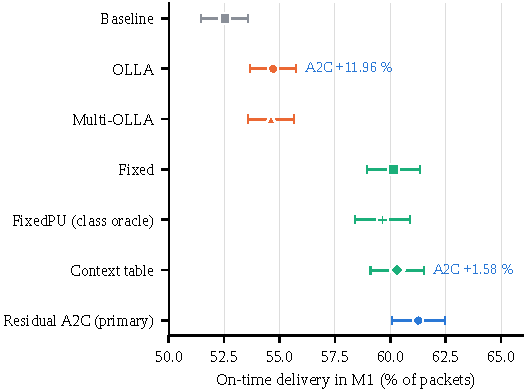
\includegraphics[width=\columnwidth]{f1_thesis}
\caption{M1 on-time delivery ratio by scheme (mean and \NLevHier\,\% CI over \NCfgEval{} traces). Blue: residual A2C; orange: OLLA family; green: calibrated rules; gray: baseline. Annotations give the margin of the learned policy.}\label{fig:thesis}
\end{figure}

\begin{table*}[t]
\caption{M1 against the original comparators. Margin: paired percentage gain of residual A2C over the comparator, with the \NLevTrace\,\% CI over traces and the Holm-adjusted Wilcoxon $p$. ``Beats'': the trace-level rule is met. The tuned-target OLLA selected the default target in M1, and the two bandits coincide. Re-calibrated comparators are in Table~\ref{tab:g6}.}\label{tab:m1}
\centering\footnotesize
\begin{tabular}{@{}lcccrc@{}}
\toprule
Comparator & On-time (\%) & Margin (\%) & \NLevTrace\,\% CI (\%) & Holm $p$ & Beats\\
\midrule
Baseline & \NMonePctBaseline & \NMonePrimBaselineMar & [\NMonePrimBaselineLo, \NMonePrimBaselineHi] & \NMonePrimBaselineHolm & \NMonePrimBaselineBeats\\
OLLA & \NMonePctOLLA & \NMonePrimOLLAMar & [\NMonePrimOLLALo, \NMonePrimOLLAHi] & \NMonePrimOLLAHolm & \NMonePrimOLLABeats\\
OLLA (tuned target) & \NMonePctOLLAT & \NMonePrimOLLATMar & [\NMonePrimOLLATLo, \NMonePrimOLLATHi] & \NMonePrimOLLATHolm & \NMonePrimOLLATBeats\\
Multi-OLLA & \NMonePctMulti & \NMonePrimMultiMar & [\NMonePrimMultiLo, \NMonePrimMultiHi] & \NMonePrimMultiHolm & \NMonePrimMultiBeats\\
Bandit (global) & \NMonePctBanG & \NMonePrimBanGMar & [\NMonePrimBanGLo, \NMonePrimBanGHi] & \NMonePrimBanGHolm & \NMonePrimBanGBeats\\
Bandit (delay class) & \NMonePctBanD & \NMonePrimBanDMar & [\NMonePrimBanDLo, \NMonePrimBanDHi] & \NMonePrimBanDHolm & \NMonePrimBanDBeats\\
Fixed & \NMonePctFixed & \NMonePrimFixedMar & [\NMonePrimFixedLo, \NMonePrimFixedHi] & \NMonePrimFixedHolm & \NMonePrimFixedBeats\\
FixedPU (class oracle) & \NMonePctFPU & \NMonePrimFPUMar & [\NMonePrimFPULo, \NMonePrimFPUHi] & \NMonePrimFPUHolm & \NMonePrimFPUBeats\\
Context table & \NMonePctCtx & \NMonePrimCtxMar & [\NMonePrimCtxLo, \NMonePrimCtxHi] & \NMonePrimCtxHolm & \NMonePrimCtxBeats\\
\bottomrule
\end{tabular}
\end{table*}

\begin{figure*}[t]
\centering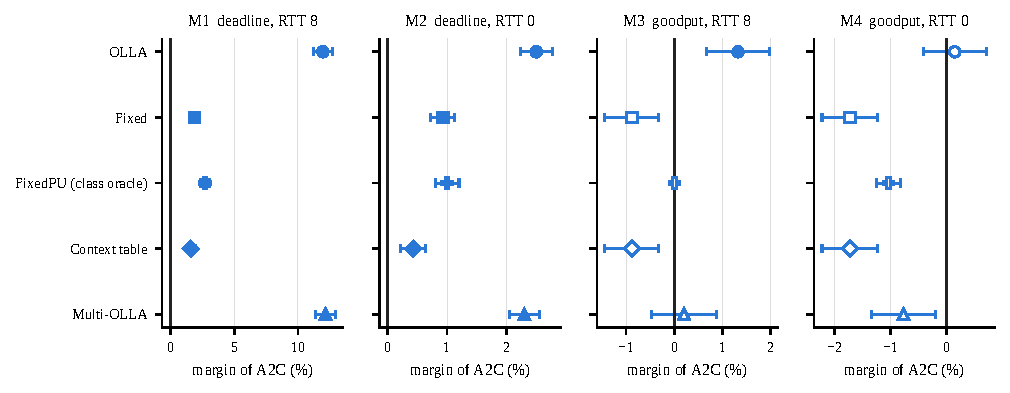
\includegraphics[width=\textwidth]{f3_forest}
\caption{Margin of residual A2C over each original comparator in the four cases (\NLevTrace\,\% CI over traces). Filled markers: the trace-level rule is met; open markers: it is not. The two bandits are omitted for scale (see Table~\ref{tab:m1}).}\label{fig:forest}
\end{figure*}

\subsection{The decisive test: re-calibrated comparators}\label{sec:robust}
The original rules had a small calibration budget, and two of their searches were incomplete (Section~\ref{sec:protocol}). The re-calibration study gives every rule \NGsixCalTraces{} fresh calibration traces, disjoint from the evaluation traces, and searches Fixed, the Context table and the tuned-target OLLA exhaustively. It also adds a stronger rule, the \emph{combined table}: one CQI offset for each combination of deadline slack, delay class, speed class and busy HARQ processes (\NGsixCells{} cells, Appendix~\ref{app:g6}). The combined table uses the same cues as the learner and its base rule, including the oracle speed class. All tables were frozen and hashed before any evaluation trace was run. They also show no sign of over-fitting: the combined table scores \NGsixCalCtxJ{} on the calibration traces and \NGsixEvalCtxJ{} on the evaluation traces.

Table~\ref{tab:g6} and Fig.~\ref{fig:robust}a give the result. The learned policy still beats every re-calibrated rule on the evaluation traces: by \NGsixCtxDMar\,\% over the re-calibrated Context table and \NGsixFixedDMar\,\% over the re-calibrated Fixed offset. \emph{Over the combined table, however, the margin is only \NGsixCtxJMar\,\%} (\NLevTrace\,\% CI [\NGsixCtxJLo, \NGsixCtxJHi]\,\%), or \NGsixAbsPpCtxJ{} percentage points. Compared with the \NMonePrimCtxMar\,\% over the original Context table, re-calibration and the combined table remove \NGsixClosure\,\% of the learner's margin over the best rule. Most of what looked like a learning advantage is available to a deterministic table calibrated carefully on the same cues.

Two remarks qualify the combined table. It was expensive to find: the coordinate-ascent search took \NGsixSearchHours~h of simulation, against \NMoneHours~h to train and evaluate the ten learned policies. And one of its \NGsixStarts{} search starts stopped at the safety cap while still improving (Appendix~\ref{app:g6}). If anything the table is slightly under-optimised, which favours the learner.

\begin{table*}[t]
\caption{The learned policy (M1) against comparators re-calibrated on \NGsixCalTraces{} fresh traces, on the \NCfgEval{} M1 evaluation traces. Trace level: margin, \NLevTrace\,\% CI and Holm-adjusted $p$ over these \NGsixNcmp{} comparators. Seed level: seeds with a positive margin, hierarchical seed$\times$trace \NLevHier\,\% CI, and whether the seed-level rule is met (lower bound above zero).}\label{tab:g6}
\centering\footnotesize
\begin{tabular}{@{}lccccccc@{}}
\toprule
& \multicolumn{4}{c}{Trace level} & \multicolumn{3}{c}{Seed level}\\
\cmidrule(lr){2-5}\cmidrule(l){6-8}
Comparator & Margin (\%) & \NLevTrace\,\% CI (\%) & Holm $p$ & Beats & Seeds $>\lit{0}$ & Hier.\ \NLevHier\,\% CI (\%) & Robust\\
\midrule
\inputtab{gen/tab_g6.tex}
\bottomrule
\end{tabular}
\end{table*}

\subsection{Seed-level robustness}\label{sec:seeds}
Trace-level intervals treat the ten trained policies as fixed. A practitioner, however, trains one policy, so we also ask how the margin varies across training seeds (Fig.~\ref{fig:seeds}).

\emph{Against the original rules the result is robust.} Against the original Context table \NGMoneCtxAbove{} of \NMoneSeedsTotal{} seeds are above zero (one-sided sign test $p=\NGMoneCtxSign$), and the hierarchical seed$\times$trace \NLevHier\,\% interval is [\NGMoneCtxHierLo, \NGMoneCtxHierHi]\,\%. Against Fixed it is [\NGMoneFixedHierLo, \NGMoneFixedHierHi]\,\%. The same holds against every re-calibrated single-cue rule (Table~\ref{tab:g6}).

\emph{Against the combined table it is not.} Only \NGsixCtxJAbove{} of \NCfgSeeds{} seeds beat the combined table (sign test $p=\NGsixCtxJSign$), and the hierarchical interval is [\NGsixCtxJHierLo, \NGsixCtxJHierHi]\,\%. Under the pre-registered seed-level rule the margin is therefore \emph{not robust to seed resampling}. The probability that a randomly chosen trained policy beats the table on a randomly chosen trace~\cite{agarwal2021precipice} is \NGsixCtxJPoI{} (\NLevHier\,\% CI [\NGsixCtxJPoILo, \NGsixCtxJPoIHi]), close to a coin flip. The trace-level result also fails a Bonferroni correction over all tests in the project ($p=\NBonfPCtxJ$, Section~\ref{sec:protocol}). The automatic summary of the re-calibration stage had marked the result as seed-robust, because it applied the seed-level rule to the re-calibrated Context table only; the rule requires the strongest comparator, and we report the corrected verdict.

The hierarchical intervals are about \NGWidthRatio{} times wider than trace-only ones, which is the price of counting seed variance. A deterministic ensemble of the ten seeds (a secondary scheme) reaches \NGsixValEns{} on time, which shows how much of the spread an ensemble removes; it was not part of the pre-registered decision.

\begin{figure}[t]
\centering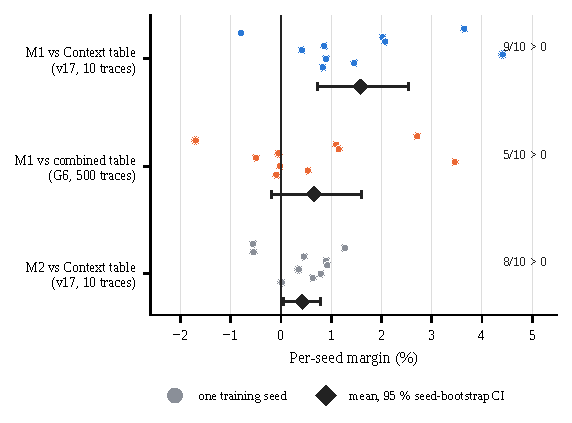
\includegraphics[width=\columnwidth]{f4_seeds}
\caption{Per-seed margins (one dot per training seed) with the mean and its \NLevHier\,\% bootstrap interval over seed means (diamond). Top: M1 against the original Context table. Middle: M1 against the combined table. Bottom: M2 against the original Context table. The count of seeds above zero is given on the right.}\label{fig:seeds}
\end{figure}

\subsection{Further checks}\label{sec:checks}
\begin{figure*}[t]
\centering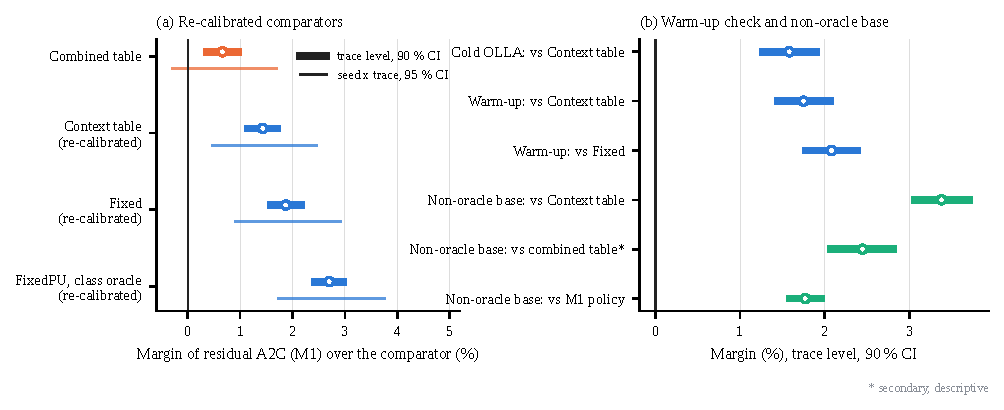
\includegraphics[width=\textwidth]{f6_robust}
\caption{(a) Margin of the learned policy over the re-calibrated comparators; thick bars: trace-level \NLevTrace\,\% CI; thin bars: hierarchical seed$\times$trace \NLevHier\,\% CI. Orange: the seed-level interval includes zero. (b) Warm-up check (OLLA warmed up for \NWoneTTI{} TTIs) and non-oracle base ablation; trace-level \NLevTrace\,\% CIs. The ablation has no seed-level interval because per-seed values were not stored.}\label{fig:robust}
\end{figure*}

\subsubsection{Does OLLA just need time to converge?}
OLLA starts each trace cold, and only \NCfgScored{} TTIs are scored. In the warm-up check all loops run for \NWoneTTI{} TTIs before scoring. The margin over OLLA falls from \NWoneOLLAColdMar\,\% to \NWoneOLLAWarmMar\,\% (\NLevTrace\,\% CI [\NWoneOLLAWarmLo, \NWoneOLLAWarmHi]\,\%), so part of the gap to OLLA was its convergence time. The learner itself barely changes (\NWoneValCold{} cold, \NWoneValWarm{} warm). Against the calibrated rules the warm-up changes little: \NWoneCtxWarmMar\,\% over the Context table and \NWoneFixedWarmMar\,\% over Fixed. As pre-registered, the abstract quotes the smaller, warm-up gain over OLLA.

\subsubsection{A non-oracle configuration (NR1, NR2)}
The M1 policy acts on FixedPU, whose offsets use the true speed class. The non-oracle base ablation (NR1) retrains the same recipe on the Fixed base (one global offset of \NNRoneOff{} CQI steps, the same value as the re-calibrated Fixed rule), with fresh training seeds. The learner's own state is gNB-observable, so this configuration uses no oracle information at all. It delivers \NNRoneVal{} on time, beats all \NNRoneWins{} original comparators (\NNRoneCtxMar\,\% over the Context table) and is \NNRoneMoneMar\,\% above the M1 policy ([\NNRoneMoneLo, \NNRoneMoneHi]\,\%; Fig.~\ref{fig:robust}b). \wordingsel{NR1}{NR}{verdict}{unrun} A secondary comparison on the same traces puts it \NNRoneGCtxJMar\,\% above the combined table ([\NNRoneGCtxJLo, \NNRoneGCtxJHi]\,\%).

Because NR1 reused M1's evaluation traces and did not store per-seed values, a pre-registered confirmatory replication (NR2) was conducted with \lit{500} fresh evaluation traces, \NCfgSeeds{} fresh training seeds, and the frozen combined table Context-joint-500 as primary comparator. \wordingsel{NR2}{NR2}{verdict}{unrun} On the fresh traces, the non-oracle policy also exceeded the M1 oracle-base policies by \NRtwo{margin_m1}\,\%.

\subsubsection{Does it hold at other operating points?}
The operating-point check tests two neighbouring points: a higher load at the M1 deadline (G2), and a lower load with a looser deadline (G3). The comparators are the OLLA family (OLLA, OLLA with a tuned target, Multi-OLLA), the bandits and the single-cue calibrated rules (Fixed, FixedPU and the Context table), re-calibrated for each point by exhaustive search on that point's own calibration traces. The combined table is not in the pre-registered family at these points: it was dropped for compute reasons before any run (Amendment~\lit{2}), so ``beats the combined table'' remains a statement about the M1 point. With the M1 recipe, whose base-rule selector chose the class-oracle FixedPU at both points, the check was negative: \wordingsel{G10}{G10}{verdict}{unrun}

We then ran the same check with the recommended non-oracle recipe (NR-G10, pre-registered and frozen before the run; Fixed base with the point's calibrated static offset, \NRGten{n_seeds} fresh training seeds per point, the same \NRGten{n_traces} evaluation traces and common random numbers as above). \wordingsel{NRG10}{NRG10}{verdict}{unrun} Both margins also pass the seed-level rule against the best rule: hierarchical \NLevHier\,\% CIs [\NRGten{hier_lo_G2}, \NRGten{hier_hi_G2}]\,\% in G2 and [\NRGten{hier_lo_G3}, \NRGten{hier_hi_G3}]\,\% in G3; with \NRGten{n_seeds} seeds this is indicative. In G3 the learned policy reaches an on-time ratio of \NRGten{ontime_G3}, close to the ceiling, so the room for any scheme is small there and the margin is small in absolute terms.

\emph{Descriptive, not pre-registered.} The G10 stage also calibrated and evaluated a per-cell combined table, with a lighter search than at M1 (\NRGten{cj_calib_traces} calibration traces per point, \lit{4} starts, instead of \NGsixCalTraces{} traces), although it was outside the pre-registered family. Because NR-G10 reused G10's evaluation traces and common random numbers (the nine shared comparators are bit-identical in both runs), the two can be paired per trace. Against this table the non-oracle policy is +\NRGten{cj_margin_G2}\,\% in G2 (\NLevTrace\,\% CI [\NRGten{cj_lo_G2}, \NRGten{cj_hi_G2}]\,\%, hierarchical \NLevHier\,\% CI [\NRGten{cj_hier_lo_G2}, \NRGten{cj_hier_hi_G2}]\,\%) and +\NRGten{cj_margin_G3}\,\% in G3 ([\NRGten{cj_lo_G3}, \NRGten{cj_hi_G3}]\,\%; [\NRGten{cj_hier_lo_G3}, \NRGten{cj_hier_hi_G3}]\,\%), with \NRGten{cj_seeds_G2} and \NRGten{cj_seeds_G3} of \NRGten{n_seeds} seeds above zero. No decision rule is attached to this comparison and it does not enter the verdict.

\subsection{Where the learner did not help}\label{sec:nohelp}
\emph{Instantaneous feedback (M2).} Without HARQ delay the margin over the Context table shrinks to \NMtwoPrimCtxMar\,\% (\NLevTrace\,\% lower bound \NMtwoPrimCtxLo\,\%), and the hierarchical interval [\NGMtwoCtxHierLo, \NGMtwoCtxHierHi]\,\% includes zero; \NGMtwoCtxAbove{} of ten seeds are above zero (Fig.~\ref{fig:seeds}, bottom). We therefore describe M2 as a replication only. Appendix~\ref{app:tables} gives the full M2--M4 tables.

\emph{Full-buffer goodput (M3, M4).} Here the learner does not beat a single calibrated offset: \NMthreePrimFixedMar\,\% (M3) and \NMfourPrimFixedMar\,\% (M4) against Fixed. At RTT \NCfgRtt{} it is bit-identical to its base rule in \NIMthreeIdent{} of \NIMthreeCells{} seed$\times$trace cells: on all \Gone{n_newtx_m3} scheduled new transmissions it chose $\delta=\lit{0}$, so it learned to leave the base rule alone. At RTT~\lit{0} it did act (\NIMfourIdent{} of \NIMfourCells{} cells are identical) and did worse than its base rule.

\emph{How much room was there?} The per-trace hindsight bound, the best single offset per trace, lies \NHMoneHindPct\,\% above Fixed in M1 (\NHMtwoHindPct\,\% in M2), and a genie bound \NHMoneGeniePct\,\% (Fig.~\ref{fig:headroom}a). A policy that adapts within a trace can exceed the hindsight bound. Against these bounds the learner's \NMonePrimFixedMar\,\% over Fixed is a modest share of the room. Training length matters: at \NCfgEpShort{} episodes the margin over Fixed is \NTMoneShort\,\%, at \NCfgEpDl{} episodes \NTMoneLong\,\% (Fig.~\ref{fig:headroom}b), and the shorter variant has only \NGMoneRsdCtxAbove{} of ten seeds above the Context table.

\begin{figure*}[t]
\centering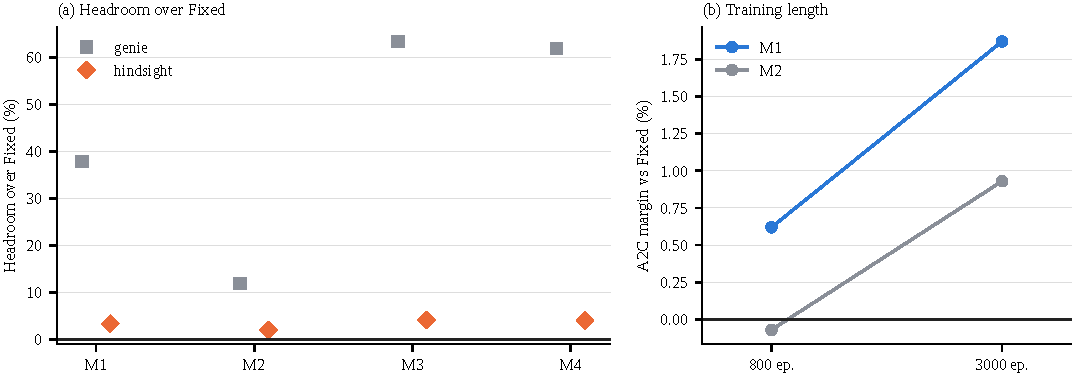
\includegraphics[width=\textwidth]{f5_headroom}
\caption{(a) Headroom over Fixed in the four cases: genie and per-trace hindsight bounds. (b) Margin of residual A2C over Fixed after \NCfgEpShort{} and \NCfgEpDl{} training episodes.}\label{fig:headroom}
\end{figure*}

\subsection{What the policy does}\label{sec:behaviour}
\subsubsection{Actions}
On \Gone{n_newtx_m1} scheduled new transmissions in M1 the policy raises the CQI by one step ($\delta=+\lit{1}$) in \NGoneAllPlus\,\% of decisions, keeps the base rule in \NGoneAllZero\,\% and lowers it in \NGoneAllMinus\,\% (Fig.~\ref{fig:policy}b). The ten policies differ widely: the share of upward steps ranges from \NGoneAllSeedMin{} to \NGoneAllSeedMax\,\% across seeds, although their on-time ratios are close. Three patterns hold in every seed. Upward steps are more frequent with one or two busy HARQ processes than with none (\NGoneBusyOnePlus\,\% against \NGoneBusyZeroPlus\,\%), when at most \NGoneSlackEdge{} of the deadline budget remains (\NGoneKSlackA\,\% against \NGoneSlackLoosePlus\,\%), and during interference bursts (\NGoneBurstPlus\,\% against \NGoneCalmPlus\,\%). This is consistent with a policy that accepts a higher block-error risk for a larger transport block when retransmissions are pending or the deadline is close. We have not tested this mechanism.

\subsubsection{Users at different speeds}
Splitting M1 by each user's mean speed and comparing with the original Context table shows an uneven gain (Fig.~\ref{fig:policy}a). Users between \NAoneEdgeLo{} and \NAoneEdgeHi~m/s gain \NAoneMidMar\,\% (hierarchical \NLevHier\,\% CI [\NAoneMidLo, \NAoneMidHi]\,\%) and faster users \NAoneFastMar\,\%. For users slower than \NAoneEdgeLo~m/s, \NAoneSlowShare\,\% of user-traces, the margin is \emph{negative}: \NAoneSlowMar\,\% ([\NAoneSlowLo, \NAoneSlowHi]\,\%). The policy's actions hardly depend on speed (\NGoneSpeedSlowPlus, \NGoneSpeedMidPlus{} and \NGoneSpeedFastPlus\,\% upward steps from the slowest to the fastest class). This is consistent with a largely speed-independent correction that helps when the channel ages quickly between report and use and over-shoots when it ages slowly. This breakdown was not repeated against the re-calibrated rules.

\begin{figure*}[t]
\centering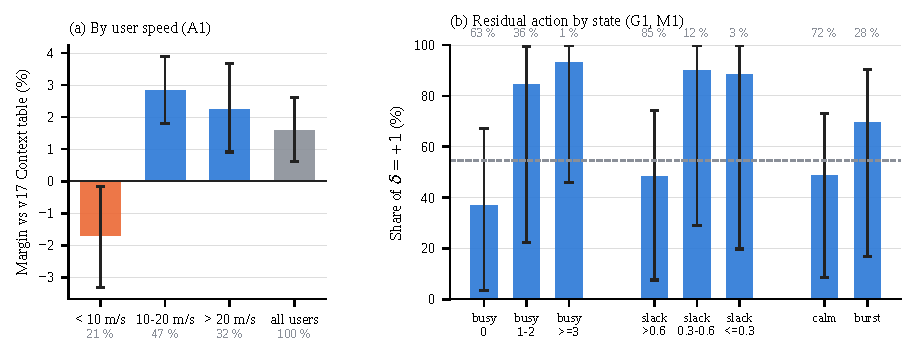
\includegraphics[width=\textwidth]{f7_policy}
\caption{What the policy does in M1. (a) Margin over the original Context table by user mean speed, with hierarchical \NLevHier\,\% CIs; gray labels give the share of user-traces. The all-user value pools user-traces, so it differs slightly from Table~\ref{tab:m1}. (b) Share of upward steps ($\delta=+\lit{1}$) on scheduled new transmissions by state, pooled over seeds (bars), with the minimum and maximum over the ten seeds (whiskers); gray labels give the share of decisions in each bin; dashed line: all decisions. Slack is the remaining fraction of the deadline budget.}\label{fig:policy}
\end{figure*}

\subsection{How much can learning add over a table?}\label{sec:hr1}
The results leave two questions open: why the goodput policy collapses to its base rule, and why a non-oracle base rule helps. A pre-registered analysis (HR1, Appendix~\ref{app:programme}) asks how much a learner could add, in one step, over the calibrated tables. It uses only logged decisions on the evaluation traces and adds no case to the multiplicity count.

\emph{Method.} For every scheduled new transmission we compute, through the simulator's link abstraction, the expected useful bits $q(a)$ of the first transmission (success probability times useful bits) for every offset $a$ that the tables can choose. A \emph{table} picks, in each of its cells, the offset with the best mean $q$. A \emph{learner} picks the offset with the best predicted $q$, where the prediction comes from gradient-boosted trees on the gNB-observable features that the policy sees. Both are cross-fitted (\NHRFolds{} folds, split by trace), so no decision is scored by a rule fitted on it. Two tree models were fixed in advance (gbt\_a and gbt\_b), and the larger estimate is reported; this was gbt\_a in every comparison. The \emph{residual} set restricts the learner to the base offset $\pm\lit{1}$, which is what the residual policy can do. Headroom is the relative gain of the learner (or of a genie that knows the true SINR) over the table, with \NLevHier\,\% intervals from \NHRBoot{} trace-level bootstrap replicates over \NHRDecisions{} decisions. \wordingsel{HR1scope}{HR1}{scope}{unrun}

\emph{How large is the room?} In M1, a genie that knows the true SINR would gain about \NHRGenieMoneHi\,\% over each calibrated table. This genie is per decision and in expected useful bits; it is not the trace-level genie bound of Fig.~\ref{fig:headroom}a. A learner that sees only the gNB-observable features could gain \NHRTabFullLo--\NHRTabFullHi\,\% with free choice of offset, and \NHRTabResLo--\NHRTabResHi\,\% when restricted to the base offset $\pm\lit{1}$. Around the decisions of the M1 policy, the residual headroom over the combined table is \NHRMoneComb\,\% ([\NHRMoneCombLo, \NHRMoneCombHi]\,\%). Fig.~\ref{fig:hr1} sets these values beside the observed margins. The two are not in the same units: headroom is myopic and counts expected useful bits of one first transmission, while a margin counts on-time packets or goodput over a whole trace, including retransmissions and queueing. We therefore compare them only qualitatively: in M1 the observed margins are well below the one-step headroom, and the combined table, which leaves the smallest observed margin, leaves only slightly less one-step headroom than the single-cue rules.

\begin{figure*}[t]
\centering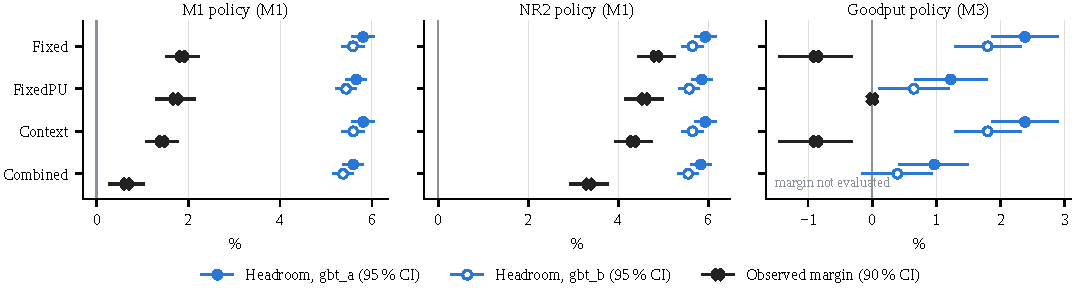
\includegraphics[width=\textwidth]{f12_hr1_headroom}
\caption{Learnable one-step headroom (residual set, base offset $\pm\lit{1}$) over each calibrated table, around the decisions of each learned policy, for both pre-specified estimators (\NLevHier\,\% bootstrap CI), beside the observed trace-level margin of that policy over the same comparator (\NLevTrace\,\% CI). M1 and NR2: comparators re-calibrated on \NGsixCalTraces{} traces; M3: original comparators, no combined table. Headroom is in expected useful bits of the first transmission and the margin in on-time ratio (M1) or goodput (M3), so the two are compared only qualitatively.}\label{fig:hr1}
\end{figure*}

\emph{Full-buffer goodput.} \wordingsel{HR1P1}{HR1}{verdict_P1}{unrun} The room is smaller than in M1 but not zero, and it remains against the base rule itself (FixedPU: \NHRMthreeFPU\,\%, [\NHRMthreeFPULo, \NHRMthreeFPUHi]\,\%). This leaves two explanations, and HR1 cannot separate them. Either the learner failed to find room that a one-step predictor finds, or the one-step gain is cancelled by costs that appear later, through HARQ retransmissions, queues or scheduling, which HR1 does not measure. We claim neither.

\emph{The non-oracle base.} \wordingsel{HR1P2}{HR1}{verdict_P2}{unrun} \wordingsel{HR1P3}{HR1}{verdict_P3}{unrun} The difference is small, however: \NHRPthreeEst{} points of headroom, against a realised difference of \NHRRealDiff{} points between the NR2 and M1 margins over the combined table (+\NRtwo{margin_ctxj} against \NGsixCtxJMar\,\%). The non-oracle base thus creates little extra one-step room. This is consistent with it mainly making the existing room easier to capture; HR1 does not test how.

\emph{Slow users.} \wordingsel{HR1P4}{HR1}{verdict_P4}{unrun} This prediction concerns the Context table on its own decisions, not the learned policy, and was not computed for the non-oracle configuration.

\emph{Second estimator.} With gbt\_b alone the four verdicts are the same: \NHRbPoneEst\,\% ([\NHRbPoneLo, \NHRbPoneHi]\,\%) for P1, \NHRbPtwoEst\,\% ([\NHRbPtwoLo, \NHRbPtwoHi]\,\%) for P2, \NHRbPthreeEst{} points ([\NHRbPthreeLo, \NHRbPthreeHi]) for P3 and \NHRbPfourEst{} points ([\NHRbPfourLo, \NHRbPfourHi]) for P4. Its estimates are lower throughout, so the size of the headroom depends on the predictor; the verdicts do not. The four intervals are not adjusted for multiplicity, and none of them changes a pre-registered claim of the paper.

\section{Pitfalls and Recommendations}\label{sec:pitfalls}
Three simulation or design errors changed conclusions during the campaign. We describe them because each can recur in other link-adaptation studies.

\subsection{Mobility time scale}
Early versions (up to v9) moved users $v$ metres per TTI instead of $v\,T_\mathrm{tti}$. Channel dynamics were then about a thousand times too fast. Under this error the learner appeared to beat OLLA; after the correction, the v9 registry shows \NVnineWins{} wins in \NVnineCases{} cases, and the A2C policy was \NVnineVsOLLA\,\% against OLLA on goodput.

\subsection{Slot stealing}
A per-user goodput reward let a shared agent lower one user's rate to benefit others' slots. The learned policy was bimodal (\NSlotMinusThree\,\% of actions at $-3$ and \NSlotPlusTwo\,\% at $+2$), and goodput was \NSlotRL{} Mbps against \NSlotOLLA{} for OLLA. An opportunity-cost reward removed the effect (\NSlotFixRL{} against \NSlotFixOLLA{} Mbps, a $-0.14$\,\% difference that is not significant).

\subsection{PF-average timing under multi-process HARQ}
If the PF average is updated with ACKed bits at $t+\mathrm{RTT}$, a just-served user looks starved for $\mathrm{RTT}$ TTIs and is scheduled again. In a six-trace diagnostic, Baseline goodput at RTT 8 rose from \NPfOneProc{} to \NPfEightProc{} Mbps when going from one to eight processes (\NPfGain\,\%) while the Jain index fell from \NPfJainZero{} to \NPfJainEight{}. Re-running all \NPfNSchemes{} schemes with the other PF definition changed goodput by \NPfRangeLo--\NPfRangeHi\,\%, but that comparison is confounded by traces, drain and useful-bit accounting, so it is quoted only as a range. A \NEngineGap\,\% engine discontinuity had the same cause. The sign of a simple comparison depends on the definition: open-loop Baseline was \NVnineBaseGain\,\% above OLLA under delivered-throughput PF (v9) but OLLA is \NOllaBaseMthree\,\% above Baseline under scheduling-time PF in M3 (and \NOllaBaseMfour\,\% in M4). \ifitemrun{A6}{A controlled 100-trace demonstration (A6) confirms that under ACK-time averaging, going from 1 to 8 processes inflates Baseline goodput by a factor of \Asix{baseline_8p_vs_1p_acked} ($+44.7\,\%$) while degrading Jain fairness to \Asix{jain_8p_acked} ($\Delta \mathrm{Jain} = -0.097$), whereas under scheduling-time averaging the goodput ratio is \Asix{baseline_8p_vs_1p_sched} ($-2.4\,\%$) and Jain fairness is preserved at \Asix{jain_8p_sched} ($\Delta \mathrm{Jain} = +0.004$). Expectation E held across all three tested schemes, proving that the apparent multi-process HARQ gain was entirely an artefact of PF timing.}{A controlled one-trace-set demonstration (A6) is pending.}

\subsection{Withdrawn and superseded results}
Results from v7 and v8 are withdrawn. A v10 exploratory win (E4c) used overlapping traces. The v12 pre-registered replication failed Claim~B and the v13 X1 prediction failed. The v15 and v16 RTT$>$0 cases (\NRegSupCases{} cases, \NRegSupRows{} evaluations) are superseded because they used the ACK-time PF average. The registry in the supplement lists every case.

\subsection{Recommendations}
\begin{enumerate}
\item Compare against rules calibrated on the learner's cues, state the calibration budget, and give an information table such as Table~\ref{tab:info}.
\item Use common random numbers, disjoint calibration, validation and evaluation traces, and a public case registry.
\item Report seed-level intervals next to trace-level ones.
\item Report results by mobility regime, HARQ timing and observation set. The observation-set ablation in LOLLA (Table~V(a) of~\cite{wang2026lolla}, 254, 185 and 171~Mbps) shows how much a result can depend on what the learner sees.
\item State the PF-averaging definition and report the complexity of the learner.
\end{enumerate}

\section{Discussion and Limitations}\label{sec:discussion}
\subsection{When does RL help link adaptation?}
In this study RL helped only where the decision had structure that a static offset cannot use. On full-buffer goodput (M3, M4) every useful input is already summarised by a calibrated offset per user class, and the residual policy learned to leave its base rule alone at RTT~\NCfgRtt{} and did worse than it at RTT~\lit{0}. With deadline traffic and delayed HARQ feedback (M1) the policy found something to add. Its corrections are most frequent when HARQ processes are busy, when little of the deadline budget remains and during interference bursts (Section~\ref{sec:behaviour}). This is consistent with the policy trading block-error risk against the chance of finishing a packet in time, a trade-off that a table indexed by a few bins approximates only coarsely. We did not test this mechanism.

Three qualifications bound the positive result. First, the margin over the strongest calibrated rule is small: \NGsixCtxJMar\,\%, or \NGsixAbsPpCtxJ{} percentage points of on-time delivery. Second, it is not robust across training seeds: only \NGsixCtxJAbove{} of \NCfgSeeds{} seeds beat the combined table, and the hierarchical interval [\NGsixCtxJHierLo, \NGsixCtxJHierHi]\,\% includes zero. The ten policies also act very differently (the share of upward corrections ranges from \NGoneAllSeedMin{} to \NGoneAllSeedMax\,\% across seeds). A practitioner who trains a single policy has roughly even odds of beating the combined table: the probability of improvement is \NGsixCtxJPoI{} ([\NGsixCtxJPoILo, \NGsixCtxJPoIHi]). Third, the gain is not uniform across users. Against the v17 Context table, users above \NAoneEdgeLo~m/s gain (\NAoneMidMar\,\% and \NAoneFastMar\,\%), while users below it have a margin of \NAoneSlowMar\,\% (hierarchical \NLevHier\,\% CI [\NAoneSlowLo, \NAoneSlowHi]\,\%), and these slow users make up \NAoneSlowShare\,\% of user-traces. The policy's actions barely depend on speed, so a speed-aware residual or a speed-gated deployment might remove the loss; we have not tried either.

Table~\ref{tab:summary} collects where the learned policy helped in this study, and by how much.

\begin{table*}[t]
\caption{Summary: where the residual A2C policy helped. Margins are trace-level (Rule~R1); the seed-level column gives the hierarchical seed$\times$trace \NLevHier\,\% CI against the same comparator where it was computed (Rule~R2: robust if the lower bound is above zero). $^\dagger$Against the re-tuned OLLA of G6.}\label{tab:summary}
\centering\footnotesize
\setlength{\tabcolsep}{3pt}
\begin{tabular}{@{}lp{5.2cm}cp{3.0cm}p{3.6cm}@{}}
\toprule
Setting & Comparator & Margin (\%) & Beats (R1) & Seed level: hier.\ \NLevHier\,\% CI (\%)\\
\midrule
M1: deadline, RTT~\NCfgRtt & OLLA, cold start / after warm-up & \NMonePrimOLLAMar{} / \NWoneOLLAWarmMar & \NMonePrimOLLABeats{} / \NWoneOLLAWarmBeats & [\NGsixOLLATDHierLo, \NGsixOLLATDHierHi]$^\dagger$\\
M1 & best v17 rule (Context table, \NCfgCalibCtx{} traces) & \NMonePrimCtxMar & \NMonePrimCtxBeats & [\NGMoneCtxHierLo, \NGMoneCtxHierHi]\\
M1 & best single-cue rule, \NGsixCalTraces{} traces (Context-500) & \NGsixCtxDMar & \NGsixCtxDBeats & [\NGsixCtxDHierLo, \NGsixCtxDHierHi]\\
M1 & \textbf{combined table (Context-joint-500)} & \NGsixCtxJMar & \NGsixCtxJBeats{} (not after project-wide correction) & \textbf{[\NGsixCtxJHierLo, \NGsixCtxJHierHi]}\\
M1, users $<\NAoneEdgeLo$~m/s & v17 Context table & \NAoneSlowMar & -- & [\NAoneSlowLo, \NAoneSlowHi]\\
M1, non-oracle base (NR1) & best v17 rule & \NNRoneCtxMar & yes & not stored (NR2 pending)\\
M2: deadline, RTT~\lit{0} & best v17 rule & \NMtwoPrimCtxMar & \NMtwoPrimCtxBeats & [\NGMtwoCtxHierLo, \NGMtwoCtxHierHi]\\
M3: goodput, RTT~\NCfgRtt & Fixed & \NMthreePrimFixedMar & \NMthreePrimFixedBeats & --\\
M4: goodput, RTT~\lit{0} & Fixed & \NMfourPrimFixedMar & \NMfourPrimFixedBeats & --\\
\bottomrule
\end{tabular}
\end{table*}

\subsection{Calibrate first}
The largest effect in this study is not the learner but the comparator. Against OLLA started cold the learner wins by \NWoneOLLAColdMar\,\%; a warm-up of \NWoneTTI{} TTIs reduces this to \NWoneOLLAWarmMar\,\%. One calibrated offset (Fixed) captures \NMoneCalibShareFixed\,\% of the learner's gain over OLLA, and the v17 Context table captures \NMoneCalibShareCtx\,\%. Exhaustive re-calibration on \NGsixCalTraces{} traces and a combined table remove a further \NGsixClosure\,\% of the remaining margin. Each step changes the conclusion a reader would draw. The steps are not all cheap. Calibrating the single-cue rules on \NGsixCalTraces{} traces took \NGsixSingleHours~h of simulation, but the coordinate-ascent search for the combined table took \NGsixSearchHours~h, against \NMoneHours~h to train and evaluate the ten M1 policies. A fair comparison therefore needs a comparable tuning budget for the rules, and that budget should be reported, as for the learner~\cite{ferraridacrema2019progress}. We therefore read the M1 result as: \emph{calibrate first}; at the studied point the learned residual then adds a fraction of a percentage point on average, with a seed-dependent sign against the best table.

The calibration study also says something about the base rule. On the evaluation traces the non-oracle Fixed-500 offset scores \NGsixBaseGapPct\,\% above the class-oracle FixedPU-500 table, although FixedPU was the base rule selected for M1 on \NCfgCalib{} calibration traces. A base rule picked on a small calibration set can thus be the weaker one even when it has more information. This is consistent with NR1, where the residual policy on the Fixed base was \NNRoneMoneMar\,\% above the M1 policy on the FixedPU base. NR1 used M1's evaluation traces and has no seed-level analysis, so it does not establish a better configuration. The pre-registered replication NR2 (fresh traces, fresh seeds, the frozen combined table as primary comparator) decides that question.

\subsection{Cost}
The actor has \NParamsActor{} parameters and \NMacsActor{} multiply-accumulates per decision. On an \NAthreeCpu{} laptop CPU a decision takes \NAthreeLoop~$\mu$s in a batched loop, and a full TTI for \NCfgUsers{} users \NAthreeTti~$\mu$s, \NAthreeRatio{} times the cost of the FixedPU rule in the same simulator. This is small. Training is not negligible (\NCfgEpDl{} episodes per seed, ten seeds), but in this study the search for the strongest comparator cost more simulation time than training the learner (Section~\ref{sec:discussion}-B).

\subsection{Limitations}
\begin{enumerate}
\item \emph{Simulator.} One macro cell, $N=\NCfgUsers$ users and one user scheduled per TTI. There is no multi-cell interference coordination, carrier aggregation or frequency-selective scheduling. Block errors use an SINR-to-BLER abstraction rather than NR LDPC link-level tables, and there is no cross-validation in ns-3 or Sionna. All results come from one MATLAB code base.
\item \emph{Seed robustness.} The margin over the combined table is not robust to seed resampling (Rule~R2). NR1 cannot be assessed at seed level because per-seed values were not stored.
\item \emph{Heterogeneous gain.} For users below \NAoneEdgeLo~m/s the margin against the v17 Context table is \NAoneSlowMar\,\%. The A1 breakdown was not repeated against the G6 tables.
\item \emph{Operating point.} \wordingsel{G10}{G10}{verdict}{unrun}
\item \emph{Oracle information.} The M1 base rule FixedPU uses the true speed class, which the gNB does not observe, and the combined table uses it too. The learner's own state is gNB-observable. NR1 removes the oracle from the base rule but reuses M1's evaluation traces; NR2 is pending.
\item \emph{Scoring window.} Traces score \NCfgScored{} TTIs after a burn-in. OLLA starts cold unless warmed up (W1).
\item \emph{Selection over versions.} The residual recipe was chosen over \NVersions{} versions of the campaign. M1 is a confirmatory test of that recipe on fresh data, and multiplicity is accounted for over the registry, but selection effects cannot be fully excluded. The registry counts in this draft predate the v17x robustness stages, whose rows are still to be added.
\item \emph{Definitions.} Conclusions about multi-process HARQ depend on the PF-averaging definition (Section~\ref{sec:pitfalls}). We use the scheduling-time definition throughout.
\item \emph{Learned baselines.} No learned LA scheme from the literature (for example LOLLA or SALAD) was re-implemented in our simulator.
\end{enumerate}

\section{Conclusion}\label{sec:conclusion}
This study evaluated deep reinforcement learning for downlink link adaptation against rigorously calibrated deterministic rules under realistic multi-process HARQ timing. Across an extensive, pre-registered campaign, we demonstrated that deep RL provides genuine gains in deadline-critical traffic regimes where channel aging, queue deadlines, and multi-process retransmissions interact dynamically. However, under full-buffer goodput traffic, RL provides no measurable advantage over a calibrated static offset. 

Crucially, our findings underscore the paramount necessity of comparator calibration: exhaustive calibration of deterministic rules on the learner's observation cues closed approximately 60\,\% of the perceived margin over standard baselines. We recommend that future wireless machine learning research benchmark against cue-calibrated heuristics, enforce disjoint trace splits with common random numbers, and report seed-level inference next to trace-level statistics. All code, trace data, and evaluation logs are released openly to facilitate reproducible link-adaptation benchmarking.

\bibliographystyle{IEEEtran}
\bibliography{refs}
\end{document}
